%\documentclass[a4paper, screen, nonacm, timestamp]{acmart}
\documentclass[acmlarge, 11pt, a4paper, screen, nonacm, timestamp]{acmart}
%\documentclass[10pt,a4paper]{article}


\usepackage{booktabs} % For formal tables

\usepackage{hyperref}
\usepackage{graphicx}
\usepackage[english]{babel}

\usepackage{xcolor}
\usepackage{url}			    	% support of \url{...}
\usepackage{listings}
\usepackage{todonotes}
\usepackage{soul}
\usepackage{longtable}
\usepackage{makecell}

\lstdefinestyle{mycpp}{
	frame=tb,
	language=C++,
	aboveskip=3mm,
	belowskip=3mm,
	showstringspaces=false,
	columns=flexible,
	basicstyle={\small\ttfamily},
	numbers=none,
	breaklines=true,
	breakatwhitespace=true
}

\lstdefinestyle{myverilog}{
	frame=tb,
	language=Verilog,
	aboveskip=3mm,
	belowskip=3mm,
	showstringspaces=false,
	columns=flexible,
	basicstyle={\small\ttfamily},
	numbers=none,
	breaklines=true,
	breakatwhitespace=true
}

\lstdefinestyle{mycmake}{
	frame=tb,
	language=make,
	aboveskip=3mm,
	belowskip=3mm,
	showstringspaces=false,
	columns=flexible,
	basicstyle={\small\ttfamily},
	numbers=none,
	breaklines=true,
	breakatwhitespace=true
}

\lstdefinestyle{mytext}{
	frame=tb,
	language=text,
	aboveskip=3mm,
	belowskip=3mm,
	showstringspaces=false,
	columns=flexible,
	basicstyle={\small\ttfamily},
	numbers=none,
	breaklines=true,
	breakatwhitespace=true
}

\lstset{frame=tb,
	language=C++,
	aboveskip=3mm,
	belowskip=3mm,
	showstringspaces=false,
	columns=flexible,
	basicstyle={\small\ttfamily},
	numbers=none,
	breaklines=true,
	breakatwhitespace=true
}

% encodings
%\usepackage[english]{babel}
%\usepackage{caption}





\begin{document}

%% Define for Intel internal document
%\newif\INTEL
 
\title[Intel Compiler for SystemC User Guide]{Intel Compiler for SystemC \\ User Guide}
\subtitle{version 1.5}

\author{Mikhail Moiseev}
\ifdefined\INTEL
\affiliation[obeypunctuation=true]{
	\institution{Intel Corporation, Intel Labs}
	\country{}
}
\else
\affiliation[obeypunctuation=true]{
	\institution{Intel Corporation }
	\country{}
}
\fi

%\email{mikhail.moiseev at intel.com}

\maketitle
\pagebreak

\setcounter{tocdepth}{2}
\tableofcontents

%\listoffigures
%\listoftables

\pagebreak

\section{Preface}

Intel\textregistered Compiler for SystemC (ICSC) is open source tool distributed under \href{https://github.com/intel/systemc-compiler/blob/main/LICENSE.txt}{Apache License v2.0 with LLVM Exceptions}. The source codes are available at \href{https://github.com/intel/systemc-compiler}{github.com/intel/systemc-compiler}.

This ICSC User Guide document intended to help user to install and run the tool, prepare SystemC design to be translated into SystemVerilog and understand the result SystemVerilog code. The User Guide document also describes some common cases in hardware design, SingleSource library of communication channels and advanced verification features.
%
There are two main documents referenced in this User Guide: 
\begin{itemize}
\item SystemC LRM -- IEEE Standard for Standard SystemC Language Reference Manual, IEEE Std 1666 2011,
\item SystemC Synthesizable Subset -- SystemC Synthesizable Subset Version 1.4.7. 
\end{itemize}

\section{Terminology and abbreviations}

In this document the following terminology is used:
%
\begin{itemize}
\item Module - SystemC module, a C++ class or structure inherits {\tt sc\_module};
\item Modular interface - SystemC module which inherits {\tt sc\_interface};
\item Record - C++ class or structure which is not module nor modular interface;
\item Signal - SystemC {\tt sc\_signal};
\item Port - SystemC {\tt sc\_in} and {\tt sc\_out};
\item Channel - signal or port;
\item Port interface - SystemC {\tt sc\_port<IF>};
\item SC vector - SystemC {\tt sc\_vector<T>}, container with objects of type {\tt T}.
\end{itemize}
%
In this document the following abbreviations are used:
%
\begin{itemize}
\item ICSC - Intel\textregistered Compiler for SystemC*;
\item SC - SystemC language;
\item SV - SystemVerilog language;
\item SVA - SystemVerilog assertions;
\end{itemize}


\include{overview}

\ifdefined\INTEL
\include{install_intel}
\else
\include{install}
\fi
\include{tool_options}

\section{Preparing SystemC design}\label{section:prepare}

\subsection{Module hierarchy}\label{section:modules}

SystemC design consists of module and modular interface instances which are organized into a module hierarchy. \emph{Module} is a C++ class or structure which inherits {\tt sc\_module} class. \emph{Modular interface} is a C++ class or structure which inherits {\tt sc\_interface} and {\tt sc\_module} classes. If a class inherits {\tt sc\_interface}, but does not inherit {\tt sc\_module} we call it \emph{pure interface}. Pure interface is not a part of module hierarchy. Each interface and module, except top module, is instantiated inside of \emph{parent module}. Modules and modular interfaces can be instantiated at stack or be dynamically allocated in heap with {\tt operator new}.

The difference between module and modular interface from ICSC viewpoint is that modular interface is flatten into parent module where it is instantiated. That means there is no modular interface instance in generated SystemVerilog, but its fields and processes are instantiated into the parent module. In other words, modular interface is a kind of module which needs to be flatten in its parent module.

The SystemC design may have one or several top module instances in {\tt sc\_main} function or another module, but only one of them will be translated into SystemVerilog. The top module to take by ICSC is specified in {\tt ELAB\_TOP} option of {\tt svc\_target}. If top module instantiated in {\tt sc\_main} function and there is no more modules instantiated, {\tt ELAB\_TOP} option could be omitted.
 
Top module contains child module(s). Every module may inherit another module(s), interface(s) or class(es) according with C++ rules. Multiple inheritance and virtual inheritance is supported by ICSC tool.

Module, interface, class or structure can be template type. Template types, template specialization and instantiation specified by C++ rules. All that is supported by ICSC tool.

In accordance with SystemC LRM, modules/modular interfaces and pointers to them cannot be function parameters, cannot be returned from function, and cannot be used as signal/port template type. 


\subsection{Module interconnect}

For inter-module communication signals, ports and port interfaces ({\tt sc\_port<IF>}) can be used. Having explicit pointers/references to another module fields or methods considered as bad programming style and should be avoided. 

Child module input/output ports could be directly connected to corresponded input/output ports of its parent module. Child ports, not connected to any signal/port, are promoted to its parent module and further up to top module. That practically means, unconnected port becomes the same type port of top module in generated SystemVerilog.

% misc_promote_ports_simple.cpp
\begin{lstlisting}[style=mycpp]
// SystemC child module port promotion to top module
SC_MODULE(Child) {
    sc_in_clk   clk{"clk"};
    sc_in<sc_int<16>>  in{"in"};       // Not connected
    sc_out<sc_int<16>> out{"out"};     // Not connected
    
    SC_CTOR(Child) {}
};

SC_MODULE(Top) {
    sc_in_clk   clk{"clk"};
    Child child_inst{"child_inst"};
    
    SC_CTOR(Top) {
        child_inst.clk(clk);
    }
};
\end{lstlisting}
%
\begin{lstlisting}[style=myverilog]
// SystemVerilog generated
module Top // "tb_inst.top_mod"
(
    input logic clk,
    input logic signed [15:0] child_instin,   // Port promoted
    output logic signed [15:0] child_instout  // Port promoted 
);
...
endmodule
\end{lstlisting}
%
Two modules with the same parent module can be connected through:
\begin{enumerate}
\item triple of sc\_in<T>, sc\_signal<T>, sc\_out<T> 
\item pair of sc\_in<T>, sc\_signal<T> 
\item pair of sc\_out<T>, sc\_signal<T> 
\end{enumerate}
%
In case (1) {\tt sc\_in<T>} port is in module A, {\tt sc\_out<T>} port in module B and {\tt sc\_signal<T>} in their parent module. These input and output ports bound to the signal in the parent module constructor.
In case (2) {\tt sc\_in<T>} port is in module A, {\tt sc\_signal<T>} in module B. The input port connected to the signal in the parent module constructor. 
In case (3) {\tt sc\_signal<T>} is in module A, {\tt sc\_out<T> }port in module B. The output port connected to the signal in the parent module constructor. 

%misc_module_binds_simple.cpp
\begin{lstlisting}[style=mycpp]
// SystemC child modules connected to each other
SC_MODULE(Producer) {
    sc_signal<bool>         req_sig{"req_sig"};
    sc_out<bool>            resp{"resp"};
    sc_out<sc_int<16>>      data{"data"};
    
    SC_CTOR(Producer) {}
};

SC_MODULE(Consumer) {
    sc_in<bool>             req{"req"};
    sc_signal<bool>         resp_sig{"resp_sig"};
    sc_in<sc_int<16>>       data{"data"};
    
    SC_CTOR(Consumer) {}
};

SC_MODULE(Parent) {
    Producer prod{"prod"};
    Consumer cons{"cons"};
    
    sc_signal<sc_int<16>>   data{"data"};

    SC_CTOR(Parent) {
        cons.req(prod.req_sig);     // in-to-signal  (2)
        prod.resp(cons.resp_sig);   // out-to-signal (3)       
        prod.data(data);            // in-to-signal-to-out (1)
        cons.data(data);
    }
};
\end{lstlisting}
%
\begin{lstlisting}[style=myverilog]
// SystemVerilog generated
module Parent // "tb_inst.top_mod"
(
);
// SystemC signals
logic signed [15:0] data;
logic resp;
logic req;

Producer prod
(
  .resp(resp),
  .data(data),
  .req_sig(req)
);
Consumer cons
(
  .resp_sig(resp),
  .req(req),
  .data(data)
);
...
endmodule
\end{lstlisting}

A module process can access its child modular interface instance fields and call methods. That is possible as interface fields and methods are moved to the parent module in generated SystemVerilog. Direct accessing fields of another module considered as bad programming style and should be avoided. 

In general case a module can have pointer to another module or {\tt sc\_port<IF>} connected to another module. It can access field and call methods of the pointee module if both of these modules are flatten in the same module in SystemVerilog. That can be parent and its child instance of modular interface or two child instances of modular interface(s) in the same parent module.

{\tt sc\_port<IF>} is special case of port which provides pure interface IF. {\tt sc\_port<IF>} can be connected to a modular interface, which implements all abstract methods of {\tt IF}. With {\tt sc\_port<IF>} it is possible to call methods of the IF that limits access to connected module. In that access via {\tt sc\_port<IF>} differs from access via modular interface pointer.

Other ways of call of another module methods or access another module fields are prohibited. 


\subsection{Module constructor and constant initialization}

Any module/modular interface must have at least one constructor. Module/modular interface constructor must have {\tt sc\_module\_name} parameter which can be passed to {\tt sc\_module} inheritor or just not used. Module/modular interface constructor can contains arbitrary C++ code. 

Module member constants can be initialized in place, in module constructor initialization list and in {\tt before\_end\_of\_elaboration} callback. Global and member constants are translated into {\tt localparam} in SystemVerilog. 
Member constants of any integral type should be 64 bit or less (stored in uint64/int64 field). Such constants with more than 64 bit has unknown value after 
elaboration, therefore error is reported.

\begin{lstlisting}[style=mycpp]
// Constants initialized in and after constructor
class MyModule : public sc_module {
    const sc_uint<8> A = 0;          // In-place initialization
    const int B[4] = {0,1,2,3};      // In-place initialization
    const bool C;       
    
    MyModule(const sc_module_name& name, int par) :
        sc_module(name), 
        C(par == 42)                 // In initialization list
    {}
    
    unsigned d;
    void setParam(unsigned par) {
       d = par;
    }
    
    const unsigned* D = nullptr;
    void before_end_of_elaboration() override {
       D = sc_new<unsigned>(d);	     // After constructor initialization
    }
}
MyModule mod("mod", 12, true);
\end{lstlisting}

Local constants in process function are translated to SV local variables. Such constants can be more than 64bit.

Non-constant module fields cannot be initialized in constructor or in place. After elaboration phase non-constant fields have unknown value. They need to be initialized in reset section of a process. 

\subsection{Method process}

Method process created with {\tt SC\_METHOD} is used to describe combinational logic, so it is \emph{combinational method} in terms of SystemC synthesizable standard. 

Method process can be sensitive to one or more signal change event or be no sensitive to any. The method sensitivity list should be static and should include all signals/ports that are read in the method function to avoid unintentional latches. ICSC tool supports latches as described in Section~\ref{section:method_latches}. 

%test_process_simple.cpp
\begin{lstlisting}[style=mycpp]
// SystemC method process example
SC_MODULE(MyModule) {
    sc_in<bool>     in{"in"};
    sc_signal<int>  sig{"sig"};
    sc_out<bool>    out{"out"};
    
    SC_CTOR(MyModule) {
        SC_METHOD(methodProc);
        sensitive << in << sig;
    }    
    void methodProc() {
    	bool b = in;        // Use in, it need to be in sensitive list
        if (sig != 0) {     // Use sig, it need to be in sensitive list
    	    out = b;
        } else {
            out = 0;
        }
    }
};
\end{lstlisting}
%
For method process ICSC generates {\tt always\_comb} block as described in~\ref{section:method_gen}.

Method process with empty sensitivity are typically used to assign constant value signal/port initialization. In the SystemVerilog code one or more {\tt assign} statements are generated for such process, see~\ref{section:empty_gen}. 

In such method it is possible to use local variables to store intermediate results. Module variable initialization can be done in such process, but not recommended as can lead to concurrent assignment to the variable. Ternary operator with arbitrary condition is supported here. {\tt if} statement with statically evaluated condition is also supported. Loops and other control flow statements cannot be used here.

Read port/signal in such method is supported, but not recommended as can lead to different behavior in Verilog vs SystemC (in SystemC process not activated if signal is changed). In the Verilog one or more assign statements are generated for method without sensitivity. 

\begin{lstlisting}[style=mycpp]
// SystemC method process with empty sensitivity
static const bool COND = true;
void emptySens()
{
    a = 0;
    if (COND) {
        b = 1;
    } else {
        c = 2;
    }
    int i = 1;
    d = (!COND) ? i : i + 1; 
}
\end{lstlisting}


\subsection{Clocked thread process}

Clocked thread process created with {\tt SC\_THREAD} and {\tt SC\_CTHREAD} macros are supported.  
Clocked thread is activated by one edge of clock signal which is specified in constructor: for {\tt SC\_CTHREAD} as second macro parameter, for {\tt SC\_THREAD} in sensitivity list. 
%
\begin{lstlisting}[style=mycpp]
// Clock thread process with clock and reset
class MyModule : public sc_module 
{
    sc_clk_in       clk{"clk"};
    sc_in<bool>     rst{"rst"};
    
	CTOR(MyModule) {
        SC_CTHREAD(threadProc, clk.pos());
        async_reset_signal_is(rst, false);
        
        SC_THREAD(threadProc);
        sensitive << clk.pos();
        async_reset_signal_is(rst, false);
	}     
}
\end{lstlisting}
%
Considering SystemC synthesizable subset restrictions on SC\_THREAD process, there is no difference between SC\_THREAD and SC\_CTHREAD processes.

Clocked thread normally has reset section and infinite loop called as \emph{main loop}. Reset section contains local variable declaration, local and module variables initialization, signal and port initialization. In reset section read of any signal/port if prohibited.

The clocked thread main loop can use any loop statements {\tt while}, {\tt for}, {\tt do...while} with \emph{true} loop condition. Main loop can contain multiple {\tt wait()} calls directly or in called functions. The main loop must contain at least one {\tt wait()} call at each path though the loop body. 
%
\begin{lstlisting}[style=mycpp]
// Clock thread with wait() in reset section and main loop
void threadProc() {
    // Reset behavior
    // ...
    wait();
    while (true) {        // Main loop
        // Operational behavior
        ...
        wait();
    }
}
\end{lstlisting}

\begin{lstlisting}[style=mycpp]
// Clock thread with one common wait() for reset and main loop
void threadProc() {
    // Reset behavior
    // ...
    while (true) {      // Main loop
        // Reset and operational behavior
        wait();
        // Operational behavior
        ...
    }
}
\end{lstlisting}

Any other loops in clocked thread may contain or not contain {\tt wait()} calls. If a loop contain a {\tt wait()} call, it must contain at least one {\tt wait()} call at each path through the loop body -- the same requirements as for main loop.
The same is true for {\tt wait(N)} calls.

There is a simple example of clocked thread. For thread process ICSC generates pair of {\tt always\_comb} and {\tt always\_ff} blocks as described in~\ref{section:thread_gen}.

\begin{lstlisting}[style=mycpp]
// SystemC simple thread example
sc_in<unsigned>    a{"a"};
sc_out<unsigned>   b{"b"};
 
CTOR(MyModule) {
   SC_CTHREAD(test_cthread, clk.pos());
   async_reset_signal_is(rst, false);
}
 
void test_cthread () {
    unsigned i = 0;
    b = 0;
    while (true) {
        wait();
        b = i;
        i = i + a;
    }
}
\end{lstlisting}

\subsection{Clock and reset}

Clocked thread process ({\tt SC\_CTHREAD} and {\tt SC\_THREAD}) is activated by one clock edge. Method process ({\tt SC\_METHOD}) can be sensitive to any change in the signals including clock positive or/and negative edge.

Method process can have arbitrary number of resets in its sensitivity list. 
\begin{lstlisting}[style=mycpp]
SC_CTOR(test_reset) {
   SC_METHOD(proc);
   sensitive << sreset << areset << ...;       
}
void proc() {
   if (!sreset || !areset) {
       // Reset behavior
   } else {
       // Normal behavior
   }
}
\end{lstlisting}

Clocked thread process can have one, several or no reset. Clocked thread cannot have more than one asynchronous reset, but can have multiple synchronous resets. SystemC synthesizable subset does not allow clocked thread without resets and multiple synchronous resets. As soon as no reset clocked threads and clocked thread with multiple synchronous resets are required for some applications that is supported by ICSC tool. 

Method process can be sensitive to all resets required.

\begin{lstlisting}[style=mycpp]
// Clocked thread with multiple resets
SC_CTOR(test_reset) {
   SC_CTHREAD(proc, clk.pos());
   reset_signal_is(sreset, true);
   async_reset_signal_is(areset, true);
   async_reset_signal_is(areset2, false);       
}

void proc() {
   enable = 0;
   wait();
   while (true) {
      wait();
   }
}
\end{lstlisting}
%
\begin{lstlisting}[style=mycpp]
// SystemVerilog generated for clocked thread with multiple resets
always_ff @(posedge clk or posedge areset or negedge areset2 /*sync sreset*/) 
begin : proc
    if (areset || ~areset2 || sreset) begin
        enable <= 0;        
    end
    else begin
        ...
    end
end
\end{lstlisting}

Clocked process without reset supported with limitations: such process can have only one {\tt wait()} and cannot have any code in reset section.

\begin{lstlisting}[style=mycpp]
// Clocked thread without reset
SC_CTOR(test_reset) {
   SC_CTHREAD(proc, clk.pos());
}

void proc() {
   while (true) {
      int i = 0;
      wait();
   }
}
\end{lstlisting}

For clocked thread process ICSC generates pair of {\tt always\_comb} and {\tt always\_ff} blocks as described in~\ref{section:thread_gen}.

There are some limitation to variable use in reset section of clocked thread described in~\ref{section:reg_in_reset}.

\subsection{Data types}

This section describes types can be used in process functions. 
SystemC integer types {\tt sc\_int}, {\tt sc\_uint}, {\tt sc\_bigint}, {\tt sc\_biguint} are supported. C++ {\tt bool}, {\tt char}, {\tt short}, {\tt integer}, {\tt long integer} and {\tt long long integer} and their unsigned versions are supported. Generated SystemVerilog data types shown in Table~\ref{tab:data_types}.

There are two special types {\tt sct\_uint<N>} and {\tt sct\_int<N>} provided. They are bit-accurate integer types which support any number of bits:
\begin{itemize}
\item {\tt sct\_int<N>} is signed integer with N bits, where N is zero or positive,
\item {\tt sct\_uint<N>} is unsigned integer with N bits, where N is zero or positive.
\end{itemize}

{\tt sct\_int<N>} and {\tt sct\_uint<N>} types automatically substitute {\tt sc\_int<N>} or {\tt sct\_bigint<N>} and {\tt sct\_uint<N>} or {\tt sct\_biguint<N>} depends on bit width. These types are implemented in {\tt sct\_sel\_types.h}.

To initialize a variable of {\tt sct\_uint<N>} type with all bits 0 or 1 there are special templates:
\begin{itemize}
\item {\tt sct\_zeros<N>} is N-bit zeros literal of {\tt sct\_uint<N>} type,
\item {\tt sct\_ones<N>} is N-bit ones literal of {\tt sct\_uint<N>} type.
\end{itemize}

\begin{lstlisting}[style=mycpp]
// Variable declaration with 0/1 initialization
sct_uint<12> a = sct_zeros<12>;
sct_uint<66> b = sct_ones<66>;
auto c  = sct_zeros<90>;
\end{lstlisting}

\begin{table}
\begin{tabular}{|l|l|l|}
\hline
SC/C++ type & SV type  & SC synthesizable subset \\
\hline
sct\_uint<N> & logic [N] & N is 0...+inf \\
sct\_int<N> & logic signed [N] & N is 0...+inf \\
sc\_uint<N> & logic [N] & N is 1...64 \\
sc\_biguint<N> & logic [N] & N is 1...+inf \\
sc\_int<N> & logic signed [N] & N is 1...64 \\
sc\_bigint<N> & logic signed [N] & N is 1...+inf \\
sc\_bv<N> & logic [N] & \\
bool & logic & \\
char, signed char & logic signed [8] & \\
unsigned char & logic [8] & \\
short & logic signed [16] & \\
unsigned short & logic [16] & \\
int & integer & 32bit \\
unsigned int & integer unsigned & 32bit \\
long & logic signed [64] & 32/64bit depends on platform \\
long long & logic signed [64] & 64bit \\
unsigned long & logic [64] & 32/64bit depends on platform \\
unsigned long long & logic [64] & 64bit \\
\_\_uint128\_t & logic [128] & \\
\_\_int128\_t & logic signed [128] & \\
\hline
\end{tabular}
\caption{Data type conversion}
\label{tab:data_types}
\end{table}

Zero width integer types {\tt sct\_int<0>} and {\tt sct\_uint<0>} intended to represent optional variables, signals, ports and record fields. In the generated SV such variables are not declared, assignment to such variable is not generated, using such variable as RValue replaced with {\tt 0}. The same works for zero width signals, ports and record fields.

\begin{lstlisting}[style=mycpp]
template <unsigned N>
struct MyModule : public sc_module {
  sct_uint<N> optVar;
  sc_in<sct_uint<N>> optInPort{"optInPort"};
  sc_signal<sct_uint<N>> optSig{"optSig"};
  struct Rec {
     sct_uint<N> optField;     
  };
}
\end{lstlisting}

Uninitialized local variable of SystemC types (sc\_uint, sc\_biguint, sc\_int, sc\_biguint) has got zero value in generated code as it got this value in the default constructor.
That means declaration of such variable leads to its initialization by {\tt 0}.

Not supported SystemC data types: {\tt sc\_lv}, {\tt sc\_logic}, {\tt sc\_signed}, {\tt sc\_unsigned}, {\tt sc\_fix}, {\tt sc\_ufix}, {\tt sc\_fixed}, {\tt sc\_ufixed}. 
Not supported floating point C++ data types: {\tt float}, {\tt double}.

C++ types can be used together with SC types. Signed and unsigned types should never be mixed, as that can lead to unexpected result for operations with negative values. For operations with mix of signed and unsigned arguments of {\tt sc\_int}/{\tt sc\_uint} types SystemC simulation can differ from generated SystemVerilog simulation. See more details in Section~\ref{section:arithmetic_gen}.



\subsection{Pointers and references}

This section describes operations with pointers and references in process functions. 
Pointers can be declared as module members and as local variables in functions. Member pointers are normally initialized at elaboration phase and used (de-referenced) in process functions. Local pointers are initialized and used in functions. Local pointers are limited to non-port/non-channel object types. 

\begin{lstlisting}[style=mycpp]
// Pointer initialization example
sc_signal<int>      s{"s"};
sc_signal<int>*     sp;
sc_signal<int>*     sd;
int   i;
int*  q;
int*  d;

SC_CTOR(MyModule){
    sp = &s;
    sd = new sc_signal<int>("sp");   
    q  = &i;
    d  = sc_new<int>();
}
void someProc() {
    int* p = d;   // Local pointer assignment in initialization
    *p = 1;
    p = q;        // ERROR, no local pointer assignment   
}
\end{lstlisting}

In module constructors there is no limitations on pointer/references and {\tt new/delete} usages. In process functions pointer de-reference ({\tt *}) operation is supported. Pointer reference ({\tt \&}) is not supported there. Operator {\tt new/new[]} and operator {\tt delete/delete[]} is not supported. Pointer assignment supported at declaration only, general pointer assignment not supported. Pointer comparison supported, other pointer arithmetic not supported. Pointer can be assigned to boolean variable, as well as, used in comparison and condition. Pointer null value ({\tt nullptr}) considered as {\tt false}, object values as {\tt true}.
Pointer function parameter supported except pointer to record which is not supported. Return value from function by pointer not supported.

\begin{lstlisting}[style=mycpp]
// Pointer arithmetic example
T   a;
T*  p = nullptr;
T*  q = &a;

void someProc() {
    bool b = !p;          // Result is true
    if (p || p == q) {    // Result is false
        ...
    }
    b = p && (*p == 1);   // De-reference pointer if its not null
}
\end{lstlisting}

Reference/constant reference type members and local variables supported. Constant reference can be initialized with variable, literal or constant expression. Reference function parameter supported. Return value from function by reference not supported. 
%
\begin{lstlisting}[style=mycpp]
// Reference example
template <class T>
T const_ref(const T& val) {
   T j = val+1;
   return j;
}

void refProc() {
  int a;
  int &b = a;             // Local reference
  b = 1;
  int i = const_ref(a);   // Parameter passed as reference
  i = const_ref(1);
}
\end{lstlisting}


\subsection{Array and SC vector types}

Arrays are supported as module members and function local variables. One-dimensional and multidimensional arrays are supported. Array of modules/modular interfaces and modules/modular interfaces pointers are supported.  In array of module/modular interface base class pointers all elements must be the same class. Array of signals/ports and signal/port pointers are supported. Array of port interfaces ({\tt sc\_port<IF>}) not supported. Array of records and record pointers are supported. In array of base class pointers all elements must be the same class.
%
\begin{lstlisting}[style=mycpp]
static const unsigned N = 5;   
static const unsigned M = 10;   
sc_uint<16>  		    a[N];
sc_in<bool>             in[N];
sc_out<sc_uint<4>>      out[N][M];
sc_signal<int>*     	sig[N];

SC_CTOR(myModule) {
  for (int i = 0; i < N; i++) {
     char sname[32];
     sprintf(sname, "sig_%d", i); 
     sig[i] = new sc_signal<int>(sname);
  }   
}
\end{lstlisting}

Array of any pointers must be homogeneous, all elements created with operator new, but not pointers to existing objects. 
Array and array of pointers, including array of signals/ports, can be a function parameter. 
 
Signal/port array index cannot be the same signal/port array. Array of record cannot be accessed at index which is the same array element.
%
\begin{lstlisting}[style=mycpp]
sc_in<T> a[N], b[M]; 
...
a[a[i]] = 0;       // Not supported 
a[b[i]] = 0;       // Supported
a[a[i].m].m = 0;   // Not supported 
a[b[i].n].m = 0;   // Supported
\end{lstlisting}

SC vector ({\tt sc\_vector}) supported for signals/ports and modules. SC vector is not supported for modular interface yet. Two-dimensional vector (vector of vectors) also supported. SC vector instances can be instantiated in modules and modular interfaces, including array of modular interfaces. SC vector cannot be passed to or returned from function.
%
\begin{lstlisting}[style=mycpp]
sc_vector<sc_in<bool>>  req{"req"};
sc_vector<sc_out<bool>> res{"resp", 3};
sc_vector<sc_vector<sc_signal<int>>> sig2d{"sig2d", 2};
SC_CTOR(MyModule) {
  req.init(3);
  sig2d[0].init(3);
  sig2d[1].init(3);        
  ...
}
\end{lstlisting}



\subsection{Record type}

This section describes usage of record which are C++ structures or classes which are not modules and modular interfaces. Records intended to represent set of plain data fields. Record can be module member as well as local variables in process functions. 

Records are supported with limitations. Record can have member functions and data members. Record member functions can contain wait() calls. Record can have members of C++/SC data types. Record cannot have another record members. Record cannot have signal/port or module/modular interface members. Record cannot have any pointer members. Record can have array members of C++/SC data types. Record cannot have array members of record. Record cannot have non-default copy/move constructors and operators.

Record can have constructor, field in-place initialization and initializer list. Record constructor can contain function calls. Record field in-place initialization and constructor initializer list cannot contain function calls.

Record can have one or multiple base classes. Record base class cannot have constructor body (constructor body should be empty), but can have initialization list and in-place initialization. Virtual functions in records are not supported.

Array of records supported. Array of pointers to record is not supported. 

Record reference supported. Pointer to record is not supported.

Record can be passed to function by value as well as by reference/constant reference, such record must have trivial copy constructor. Record can be returned from function by value, such record must have trivial copy constructor.
%
\begin{lstlisting}[style=mycpp]
// Simple record example
struct Rec1 {
    int x;
    sc_int<2> y;
};
// Record with constructor
struct Rec2 {
    sc_uint<16> a;       
    bool b;
    Rec2(int i) : b(i == 42) {
        a = i + 1;
    }
};
\end{lstlisting}

Record declaration with and without parameters supported in the following forms:
%
\begin{lstlisting}[style=mycpp]
Rec1 r1;        	// OK
Rec1 r1();        	// OK
Rec1 r1{};        	// OK
Rec1 r1 = Rec1{}; 	// Error
Rec1 r1 = Rec1();  	// Error
Rec2 r2(42);    	// OK
Rec2 r2{42};    	// OK
\end{lstlisting}

Signal and port of record type are supported. Record used as signal and ports type should have a constructor without parameters. This constructor is used for the signal/ports initialization. Such a record should have {\tt operator==()} and {\tt operator<<(std::ostream)} and {\tt sc\_trace()} defined.
Signal and ports of record can be read/written and assigned to a record variable.
%
\begin{lstlisting}[style=mycpp]
struct SRec {
    int x;
    sc_int<2> y;
    bool operator == (const SRec& other) {
        return (x == other.x && y == other.y);
    } 
};
::std::ostream& operator << (::std::ostream& os, const SRec& s) {
    os << s.x << s.y;
    return os;
}
...
sc_in<SRec>     in{"in"};
sc_out<SRec>    out{"out"};
sc_signal<SRec> s{"s"};
...
SRec r1;          // OK
r1 = in.read();   // OK
r1 = s;           // OK
s = Rec1();       // OK
s.write(r1);      // OK
out = r1;         // OK
out = Rec1{};     // OK
int x = in.read().x;   // OK
\end{lstlisting}
 
Code generation rules for record described in Section~\ref{section:record_gen}. 

\subsection{Union type}

Union type not supported.

\subsection{Type cast}

This section describes type cast operations can be used in process functions. 

Type cast in C style ((T)x), functional style (T(x)), and static cast supported for right side of assignment statement and function arguments. Type cast for left side of assignment is ignored. 
Constant cast {\tt const\_cast} is prohibited in left part of assignment, and ignored elsewhere. Reinterpret and dynamic type casts are not supported.

Type cast can be used to change width or/and signness of the variable, literal or expression. 
Type cast to change unsigned object to signed is supported in binary, unary and compound operations. In other operations type cast to signed as well as all type casts to unsigned are ignored. 

Multiple casts for one object are supported. 
SystemC type conversion to C++ integer methods {\tt to\_int(), to\_uint()}, {\tt to\_long(), to\_ulong(}), {\tt to\_int64(), to\_uint64()} supported. 
%
% method_cast.cpp
\begin{lstlisting}[style=mycpp]
int i;
bool b;
sc_uint<4> x;
sc_uint<8> y;
b = (bool)i; 
i = x.to_int();
y = (sc_uint<3>)x;
y = (sc_uint<6>)((sc_uint<2>)x);
\end{lstlisting}
%
\begin{lstlisting}[style=myverilog]
b = |i;
i = 32'(x);
y = 3'(x);
y = 6'(2'(x));
\end{lstlisting}

Type cast to cast negative value to unsigned is prohibited. Type cast unsigned with set high bit to signed negative is prohibited.
%
% method_cast.cpp
\begin{lstlisting}[style=mycpp]
unsigned u = 0x1FFFFFFFFUL;
int i = -1;
long l = (int)u;                    // Prohibited as result is negative value
unsigned long ul = (unsigned)i;     // Prohibited as operand has negative value
\end{lstlisting}

Type cast to base class supported for function call (T::f()) and member access (T::m).


\subsection{Dynamic memory allocation}

Dynamic memory allocation is supported at elaboration phase only, i.e. in module constructors and functions called from there. Dynamic memory allocation not supported in process functions.

Dynamic allocation supported for all types including modules, interfaces, signals and ports. That is also supported for array of pointers to modules, interfaces, signals and ports.

ICSC uses dynamic elaboration that provides arbitrary C++ code support at elaboration phase, but not able to distinguish between pointer to dynamically allocated object and dangling pointer. To solve this problem ICSC uses overriding operators {\tt new} and {\tt new[]}. For modules, interfaces, signals, ports and other inheritors of {\tt sc\_object} operators {\tt new} and {\tt new[]} overridden in the patched SystemC library used by ICSC. 

For dynamic memory allocation for non-{\tt sc\_object} types, like C++ types, there are special functions {\tt sc\_new} and {\tt sc\_new\_array}. {\tt sc\_new} is used for scalar types instead of {\tt new}, {\tt sc\_new\_array} used for arrays instead of {\tt new[]}. {\tt sc\_new} and {\tt sc\_new\_array} declarations:
%
\begin{lstlisting}[style=mycpp]
template<class T, class... Args>
T* sc_new(Args&&... args);
 
template<class T>
T* sc_new_array(size_t array_size);
\end{lstlisting}

Using {\tt sc\_new} and {\tt sc\_new\_array} examples:
% 
% misc_module_section.cpp
\begin{lstlisting}[style=mycpp]
struct MyRec {
  int i;
  MyRec(int i_) : i(i_) {};
};
sc_signal<bool>* ap;
bool* bp;
sc_uint<8>* vp;
MyRec* mp;
sc_in<int>** ports;
sc_signal<int>* signals;
   
SC_MODULE(MyModule) {
  ap = new sc_signal<bool>("a");     // OK, signal is sc_object
  bp = new bool;                     // ERROR, non-sc_object
  bp = sc_new<bool>();               // OK
  vp = new sc_uint<8>();             // ERROR, non-sc_object
  vp = sc_new<sc_uint<8>>();         // OK
  mp = new MyRec(42);                // ERROR, new for non-sc_object
  mp = sc_new<MyRec>(42);            // OK, using sc_new
  ports = new sc_in<int>* [10];      // ERROR, new for pointer, non-sc_object 
  ports = sc_new_array<sc_in<int>*>(10);    // OK, using sc_new_array
  signals = new sc_signal <int>[10];        // OK, array of sc_objects 
};
\end{lstlisting}


\subsection{Control flow operators}

All control flow operators are supported. 
Conditions of {\tt if}, {\tt ?}, {\tt for}, {\tt while}, {\tt do..while} should be expression without side effects. Complex conditions with {\tt ||}, {\tt \&\&}, {\tt !} and brackets supported. If left part of logical expressions with {\tt ||} and {\tt \&\&} evaluated as constant, right part code is not generated. 
%
That allows to check pointer is not null and do the pointer de-reference it in the condition expression. {\tt if} and {\tt ?} conditions, including complex conditions, can contain function call without side effects and without {\tt wait()}. {\tt for}, {\tt while}, {\tt do..while} conditions cannot have any function call.

There are two kind of synthesizable loops:
\begin{enumerate}
\item loop without {\tt wait()/wait(N)}, for these loops iteration number must be statically determinable,
\item loop with {\tt wait()/wait(N)}, for these loops iteration number may be unknown.
\end{enumerate}


\subsubsection{if}

{\tt if} statement is translated into SystemVerilog {\tt if}. 

\begin{lstlisting}[style=mycpp]
// Operator if examples
if (a || b) {...}
if (true || a) {...}
if (false && b) {...}
\end{lstlisting}
%
\begin{lstlisting}[style=myverilog]
// SystemVerilog generated for if example
if (a || b) begin 
    ... 
end
if (1) begin 
    ... 
end
if (0) begin     // Empty if generated
end
\end{lstlisting}

\subsubsection{switch}

{\tt switch} statement is translated into SystemVerilog {\tt case}, see Section~\ref{section:switch_gen}.
{\tt switch} statement can have one or more cases including optional {\tt default} case. Each case must have one and only one final {\tt break} as the last statement of the case. {\tt default} case also must contain final {\tt break}. Another option is empty case or empty {\tt default} case. For empty case the next non-empty case (possibly {\tt default} case) code is copied in the generated SV.

{\tt switch} case code can contain if/loop statements as well as inner switch statements. {\tt switch} case code can contain function calls. {\tt switch} statement in called function can contains {\tt return} statements in the end of all cases. For such {\tt switch} cases final {\tt break} statement not allowed, no mix of {\tt return} and {\tt break} supported.

\begin{lstlisting}[style=mycpp]
// Operator switch example
switch (i) {
case 0: i++; break;
case 1: i--; break;
default: i = 0; break;
}
\end{lstlisting}


{\tt switch} statement in called function can contain {\tt return} statements in the end of all cases. For such {\tt switch} no {\tt break} statements required.

\begin{lstlisting}[style=mycpp]
// Operator switch in function example
void f() {
    ...
    switch (i) {
    case 0: i++; return;
    case 1: i--; return;
    }
    return;
}
\end{lstlisting}


\begin{lstlisting}[style=mycpp]
// Operator switch with empty case
switch (i) {
case 0: 
case 1: k = 1; break;
default: k = 2; break;
}
\end{lstlisting}


\subsubsection{for}

{\tt for} statement is translated into SystemVerilog {\tt for} or into {\tt if} see Section~\ref{section:loop_thread}. 

{\tt for} loop can have only one counter variable with optional initialization, condition and increment sections. The variable can be declared in the loop initialization. 
Initialization section can have simple variable initialization or assignment only, cannot have function call.
Condition section can have one comparison operator for the loop variable, cannot have function call.
Increment section can have increment or decrement of the loop variable, cannot have function call. 

Several examples of correct {\tt for} loop is given in the following listing:
%
\begin{lstlisting}[style=mycpp]
// Operator for examples
const unsigned N = 10;
for (int i = 0; i < N; i++) {...}

int i = N;
for (; i != 0; --i) {...}

int j = 0;
for (; j < N; ) {...}
\end{lstlisting}

\subsubsection{while}

{\tt while} statement is translated into SystemVerilog {\tt while} or into {\tt if} see Section~\ref{section:loop_thread}.
{\tt while} condition is an arbitrary expression without function call.
Several examples of correct {\tt while} loop is given in the following listing:
%
\begin{lstlisting}[style=mycpp]
// Operator while examples
const unsigned N = 10;
int i = 0;
while (i < N) {...}

int j = N;
int k = 0;
while (j != 0 && j != k) {...}

// Waiting for enable, this while loop should contain wait() at each path
while (!enable.read()) {...}
\end{lstlisting}

\subsubsection{do...while}

{\tt do..while} statement is translated into SystemVerilog {\tt do..while} or into {\tt if} see Section~\ref{section:loop_thread}. 
{\tt do..while} condition is an arbitrary expression without function call.
Several examples of correct {\tt do..while} loop is given in the following listing:
%
\begin{lstlisting}[style=mycpp]
// Operator do..while examples
const unsigned N = 10;
int i = 0;
do {
   ...
} while (i < N);

int j = N;
int k = 0;
do {
   ...
} while (j != 0 && j != k);
\end{lstlisting}

\subsubsection{break}

{\tt break} statement is translated into SystemVerilog {\tt break} or substituted  with code after the loop body, see Section~\ref{section:loop_thread}. 

\subsubsection{continue}

{\tt continue} statement is translated into SystemVerilog {\tt continue} or substituted with code in the loop body, see Section~\ref{section:loop_thread}. 

\subsubsection{goto}

Not supported.

\subsection{Function calls}

This section describes functions and function calls rules. Module/modular interface/record static and non-static functions supported. Global/namespace functions supported. Recursive functions not supported.

Function can have parameters and returned value. Function can have local variable of non-channel type. Local variables can be non-static or constant static. No static non-constant local variables allowed.

Function parameters can be passed by value, by reference reference, and by pointer, including pointer to channel. Constant reference parameter argument can be literal of the corresponding type.
Function can return result by value only. Return by reference or by  pointer not supported. Function with return type {\tt void} can use {\tt return} statement without argument. 
%
% method_fcall.cpp
\begin{lstlisting}[style=mycpp]
// No parameters function
void f1() {
   m = m + 1;
}       
// Parameters passed by value 
int f2(int i, bool b = false) {
  return (b) ? i : i+1;
}    
// Parameters passed by reference 
void f3(int& i) {
  i++;
}
// Parameters passed by pointer
unsigned f4(sc_uint<16>* i) {
  return (*i+1);
}
// Array passed 
int f5(int arr_par[3]) {
  int res = 0;
  for (int i = 0; i < 3; i++) {
    res += arr_par[i];
  }
  return res;
}
\end{lstlisting}

Function with multiple {\tt return} supported. Function {\tt return} statement(s) is replaced with function result to variable assignment in SV code.  That leads to a function must have no code after {\tt return}. In particular, {\tt return} statement in loop is not supported.  Function with return type void can have {\tt return} statement(s) without argument. For {\tt return} statement without argument no code is generated.
%
% method_fcall.cpp
\begin{lstlisting}[style=mycpp]
// Multiple returns
int f6(int& val) {
  if (val) {
     return 1;
  } else {
     return 2;
  }
}
// Multiple returns in switch
unsigned f7(unsigned val) {
   switch (val) {
     case 1: return 1;
     case 2: return 2;
     default: return 3;
   }
}
\end{lstlisting}

Module member function can access this module fields/functions and child modular interface instance(s) fields/functions. Access to child modular interface instance members allowed through a port interface ({\tt sc\_port<IF>}) or a pointer to the modular interface. The accessed modular interface is flatten in module/modular interface with does access to it, see~\ref{section:modules}.

Virtual functions supported. Function overload and hide function in child class supported.


\subsection{Naming restrictions}

Prefixes {\tt sct\_} and {\tt SCT\_} are used for special function and cannot be used in user SystemC code.
Suffix {\tt \_next} is used for register variables, so it is not recommended to use such suffix for SystemC variables.

ICSC tool provides {\tt \_\_SC\_TOOL\_\_} define for input SystemC project translation. 
Module/interface field {\tt\_\_SC\_TOOL\_MODULE\_NAME\_\_} is reserved for vendor memory name. 
Module/interface field {\tt \_\_SC\_TOOL\_VERILOG\_MOD\_\_} is reserved for disable module generation in SystemVerilog code. 



\section{SystemVerilog generation rules}\label{section:trans_flow}

This section describes how C++/SystemC modules, processes, functions, declarations, statements and expressions are translated into SystemVerilog code.
For an input SystemC design ICSC generates one output SystemVerilog file with all the modules inside.


\subsection{Module generation}\label{section:module_gen}

Module hierarchy generation started with top module and passed through all the child modules. For any module there are multiple SV code sections generated:
\begin{itemize}
\item Input and output ports;
\item Variables generated for SystemC signals;
\item Local parameters generated for C++ constants;
\item Assignments generated for SystemC array of channels;
\item Process variables and always blocks;
\item Child module instances;
\item SVA generated for SystemC temporal assertions.
\end{itemize}

Assignments for SystemC array of channels provides conversion of array elements to individual channels in module interface. That is required if individual array elements bound to different channels. In case array of channels is bound to other same size array of channels, module interface contains array of channels and no assignments required. 

There is an illustrative example for module with all the sections generated:
%
\begin{lstlisting}[style=mycpp]
// Module structure example
SC_MODULE(MyChild) {...};

SC_MODULE(MyModule) {
    sc_in_clk               clk{"clk"};
    sc_in<sc_uint<4>>       a{"a"};
    sc_out<sc_int<5>>       b{"b"};
    sc_in<bool>             f[2];    
    
    sc_signal<bool>         s{"s"};
    sc_signal<sc_uint<32>>  t{"t"};
    
    MyChild                 m{"m"};    
    
    static const bool C = true;
    static const int  D = 42;
    
    SC_CTOR(MyModule) {
        SC_CTHREAD(threadProc, clk.pos());
        async_reset_signal_is(rst, 0);
    }    
    
    void proc() {
       ...
    }
};
\end{lstlisting}
%
\begin{lstlisting}[style=myverilog]
// Generated SystemVerilog
// Input and output ports
module MyModule // "tb_inst.top_mod"
(
    input logic clk,
    input logic [3:0] a,
    output logic signed [4:0] b,
    input logic f0,
    input logic f1
);

//------------------------------------------------------------------------------
// Variables generated for SystemC signals
logic s;
logic [31:0] t;
logic f[2];

//------------------------------------------------------------------------------
// Local parameters generated for C++ constants
localparam logic signed C = 'd1;
localparam logic signed [31:0] D = 'd42;

//------------------------------------------------------------------------------
// Assignments generated for SystemC channel arrays
assign f[0] = f0;
assign f[1] = f1;

//------------------------------------------------------------------------------
// Process variables and always blocks
// Thread-local variables
logic [31:0] t_next;
// Next-state combinational logic
always_comb begin : threadProc_comb     // test_module_sections.cpp:89:5
...
end
// Syncrhonous register update
always_ff @(posedge clk or negedge rst) 
begin : threadProc_ff
...
end

//------------------------------------------------------------------------------
// Child module instances
MyChild m
(
  ...
);

//------------------------------------------------------------------------------
// SVA generated for SystemC temporal assertions
`ifndef INTEL_SVA_OFF
sctAssertLine55 : assert property (...)
`endif // INTEL_SVA_OFF
endmodule
\end{lstlisting}

\subsection{Variables generation}\label{section:var_gen}

There are several types of variables used in SC process functions: local variables (non-channel only), member non-channel variables, member channel variables. For these types of SC variables different types of SV variables are generated depends on variable usages. 

Non-channel variable can be generated as a register or as a combinational variable. In clocked thread process:
%
\begin{itemize}
\item If non-channel variable defined before read after last {\tt wait()/wait(N)} at every path, it is combinational variable;
\item If non-channel variable can be read before defined after last {\tt wait()/wait(N)}, it is register variable.
\end{itemize}
%
In method process only combinational variables are generated. That is because a  non-channel variable must be defined before used. 

Channel variable can be generated as an input or a register:
%
\begin{itemize}
\item If channel variable is never assigned, it is an input (no register);
\item If channel variable is assigned at least once, it is a register.
\end{itemize}
%
If a signal/port register is not initialized in reset section, warning is reported.

Register in generated code consists of two variables: \emph{current value} and \emph{next value}. The current value variable is updated in {\tt always\_ff} block with next value variable. The next value variable is updated in {\tt always\_comb} block with current value variable.

In the following example, local variable {\tt j} there will be {\tt j} and {\tt j\_next} SV variables generated. SV variable {\tt j} stores old value of the variable, assigned at last process activated cycle. {\tt j\_next} stores a new value assigned in the current cycle.

\begin{lstlisting}[style=mycpp]
sc_out<int>    a;   // Member channel
sc_signal<int> b;   // Member channel
int c;              // Member non-channel
int d;              // Member non-channel

void threadProc() {
    int j = 0;          
    a = 0;
    c = 0;
    d = 1;
    wait();

    while (true) {
        a = j;                  // Channel a is defined
        int i = 0;              // Local j is defined before use
        j = b + i;              // Local j is used before define
        c = b;                  // Non-channel c is defined before use
        i = a.read() + c + d;   // Local i is not used
        d = a.read();           // Non-channel d is used before define
        wait();
    }
}
\end{lstlisting}
%
\begin{lstlisting}[style=myverilog]
// SystemVerilog generated
module MyModule // "tb_inst.top_mod"
(
    ...
    output logic signed [31:0] a
);

// Thread-local variables
logic signed [31:0] a_next;
logic signed [31:0] j;
logic signed [31:0] j_next;
logic signed [31:0] d;
logic signed [31:0] d_next;
logic signed [31:0] c;

// Next-state combinational logic
always_comb begin : threadProc_comb     // test_module_sections.cpp:89:5
    threadProc_func;
end
function void threadProc_func;
    integer i;
    a_next = a;
    d_next = d;
    j_next = j;
    a_next = j_next;
    i = 0;
    j_next = b + i;
    c = b;
    i = a + c + d_next;
    d_next = a;
endfunction

// Syncrhonous register update
always_ff @(posedge clk or negedge rst) 
begin : threadProc_ff
    if ( ~rst ) begin
        integer c;
        j <= 0;
        a <= 0;
        c = 0;
        d <= 1;
    end
    else begin
        a <= a_next;
        j <= j_next;
        d <= d_next;
    end
end
\end{lstlisting}

\subsection{Non-modified member variables generation}\label{section:non_modif_var_gen}
Module or modular interface member variables which are non-modified in any process, considered as initialized at elaboration phase. Because of dynamic elaborator used in the tool, it is not possible to detect if a variable is not initialized at elaboration phase. 

For such member variables which are scalar (non-array) and non-record type, SV local parameters are generated. 
No local parameters generated for array and record members, so these variables remain non-initialized. Such member variable should be initialized in reset section of a process where it is used.

\begin{lstlisting}[style=mycpp]
class MyModule : public sc_module {
  	bool C = true;
	int D;
   	unsigned E;

	CTOR (MyModule) {
   		D = 42;
	}
	void setE(unsigned par) { E = par; }
}
...
MyModule m{"m"};
...
m.setE(43);   // In parent module constructor
\end{lstlisting}
%
\begin{lstlisting}[style=myverilog]
// Generated SystemVerilog
localparam logic C = 1;
localparam logic signed [31:0] D = 42;
localparam logic [31:0] E = 43;
\end{lstlisting}

Nothing is generated if the variable is not used in any process. If such variable is member of array of modular interfaces, it should be used in a process of each modular interface.

\subsection{Constants generation}\label{section:const_gen}

For constants and static constants SV local parameters are generated.

\begin{lstlisting}[style=mycpp]
static const bool C = true;
static const int D = 42;
\end{lstlisting}
%
\begin{lstlisting}[style=myverilog]
// Generated SystemVerilog
// C++ constants
localparam logic signed C = 'd1;
localparam logic signed [31:0] D = 'd42;
\end{lstlisting}

There is {\tt REPLACE\_CONST\_VARIABLES} option to replace the constants in the code with their values, see~\ref{section:tool_options}. A constant is replaced with its value if the value if there is no reference to the constant. If constant is replaced with its value or not used in the code, no SV local parameter is generated.

\subsection{Integer variable initialization from string}\label{section:string_to_int}

Integer variable of SC type ({\tt sc\_uint}, {\tt sc\_int}, {\tt sc\_biguint}, {\tt sc\_bigint}) can be initialized from string literal or string variable. The string should contain correct integer value in any radix supported. For {\tt sc\_biguint} and {\tt sc\_bigint} initialization value could be more than 64 bits. String variable should be initialized at elaboration phase (in a module constructor).

\begin{lstlisting}[style=mycpp]
const char* cstr = "43";
std::string str;                    // Initialized in constructor or a method call

void someProc() {
    sc_uint<16> ux = "0b110011";    // Initialization with string literal
    ux = "42";                      // String literal assignment    
    ux = sc_uint<5>("0x42");        // Cast at initialization supported
    ux = cstr;                      // C string assignment
    ux = str.c_str();               // std::string assignment
    sc_biguint<65> bu;  
    bu = "0x1FFFF1111FFFF1111";     // More than 64bit literal
}
\end{lstlisting}

\subsection{Method process generation}\label{section:method_gen}

Method process is directly translated into {\tt always\_comb} block. All the local variables of the method are translated into local variables in the {\tt always\_comb} block. 

\begin{lstlisting}[style=mycpp]
// Method process example
void methodProc() {
    bool x;
    int i;
    i = a.read();
    x = i == b.read();
    sig = (x) ? i : 0;
}
\end{lstlisting}

\begin{lstlisting}[style=myverilog]
// SystemVerilog generated for method process example
always_comb 
begin : methodProc     // test_module_sections.cpp:110:5
    logic x;
    integer i;
    i = a;
    x = i == b;
    sig = x ? i : 0;
end
\end{lstlisting}

\subsection{Method process with empty sensitivity}\label{section:empty_gen}

Method process with empty sensitivity are typically used to assign constant value signal/port initialization. In the SystemVerilog code one or more {\tt assign} statements are generated for such process. 

\begin{lstlisting}[style=mycpp]
// SystemC method process with empty sensitivity
static const bool COND = true;
void emptySens()
{
    a = 0;
    if (COND) {
        b = 1;
    } else {
        c = 2;
    }
    int i = 1;
    d = (!COND) ? i : i + 1; 
}
\end{lstlisting}
%
\begin{lstlisting}[style=myverilog]
// SystemVerilog generated
assign a = 0;
assign b = 1;
assign i = 1;
assign d = i+1;
\end{lstlisting}


\subsection{Method process with latch(es)}\label{section:method_latches}

Normally ICSC does not allow to have latch in SystemC source, but there are some cases where latch is required. There is ICSC assertion {\tt sct\_assert\_latch} which intended to specify latch in method process, see~\ref{section:assert_special}. It suppresses ICSC error message for latch variable, signal or port. 

Normal method process translated into {\tt always\_comb} block in SystemVerilog. For method with latch {\tt always\_latch} block is generated.

\begin{lstlisting}[style=mycpp]
// SystemC source for Clock Gate cell
#include "sct_assert.h"
void cgProc() {
    if (!clk_in) {
        enable = enable_in;
    }
    // To prevent error reporting for latch
    sct_assert_latch(enable);
}
void cgOutProc() {
    clk_out = enable && clk_in;
}
\end{lstlisting}
%
\begin{lstlisting}[style=myverilog]
// SystemVerilog generated 
always_latch
begin : cgProc
    if (!clk_in) begin
        enable <= enable_in;
    end
end
\end{lstlisting}

\subsection{Thread process generation}\label{section:thread_gen}

Clocked thread process in SystemC has one or multiple states specified with {\tt wait()}/{\tt wait(N)} calls, therefore it cannot be directly translated into {\tt always\_ff} block. 
To translate semantics of multi-state thread into a form which is accepted by most SystemVerilog tools, ICSC converts the thread into pair of {\tt always\_comb} and {\tt always\_ff} blocks. {\tt always\_ff} block implements reset and update logic for state register and other registers. {\tt always\_comb} block contains combinational logic that computes the next state. {\tt always\_comb} contains all the logic of the SystemC thread and provides combinational outputs which are stored into registers in the {\tt always\_ff} block. 

Thread states are identified by {\tt wait()} call statements in the SystemC code, so number of states is the number of {\tt wait()} calls, including such in called functions. {\tt wait(N)} calls are discussed in~\ref{section:waitn_gen}. 

For thread process with one state, generated {\tt always\_comb} block has all the after-reset logic.

For thread with multiple states, generated {\tt always\_comb} block has main {\tt case} for thread process states. The main {\tt case} branches correspond to SystemC code that starts from specific {\tt wait()} and finishes in the next {\tt wait()}. Implicit thread states are represented by automatically generated {\tt PROC\_STATE} variable with process name prefix. 

\begin{lstlisting}[style=mycpp]
// Thread process example
void multiStateProc() {
   sc_uint<16> x = 0;
   sig = 1;              
   wait();                    // STATE 0

   while (true) {
      sc_uint<8> y = a.read(); 
      x = y + 1;
      wait();                 // STATE 1
      sig = x;           
   }
}
\end{lstlisting}

\begin{lstlisting}[style=myverilog]
// SystemVerilog generated for thread process example
// Thread-local variables
...
logic multiStateProc_PROC_STATE;
logic multiStateProc_PROC_STATE_next;

// Next-state combinational logic
always_comb begin : multiStateProc_comb     // test_module_sections.cpp:122:4
    multiStateProc_func;
end
function void multiStateProc_func;
    logic [7:0] y;
    sig_next0 = sig;
    x_next = x;
    multiStateProc_PROC_STATE_next = multiStateProc_PROC_STATE;
    
    case (multiStateProc_PROC_STATE)
        0: begin
            y = a;
            x_next = y + 1;
            multiStateProc_PROC_STATE_next = 1; return;  
        end
        1: begin
            sig_next0 = x_next;
            y = a;
            x_next = y + 1;
            multiStateProc_PROC_STATE_next = 1; return; 
        end
    endcase
endfunction

// Syncrhonous register update
always_ff @(posedge clk or negedge rst) 
begin : multiStateProc_ff
    if ( ~rst ) begin
        x <= 0;
        sig <= 1;
        multiStateProc_PROC_STATE <= 0;  // test_module_sections.cpp:125:8;
    end
    else begin
        sig <= sig_next0;
        x <= x_next;
        multiStateProc_PROC_STATE <= multiStateProc_PROC_STATE_next;
    end
end
\end{lstlisting}

\subsection{Register variables in thread reset section}\label{section:reg_in_reset}

There are some limitations to use register variables in reset section of clocked thread. Register variable is a variable which keeps its values between thread states. Register variable {\tt i} is represented with a pair of variables {\tt i} and {\tt i\_next} in SV code. Register next to current value has non-blocking assignment in {\tt always\_ff} block, therefore such variable cannot have blocking assignment in reset section. For operations which modify register variable in reset section error is reported:
%
\begin{lstlisting}[style=mycpp]
void proc() {
    int i = 1;      // Register variable
    i++;            // Error reported
    i += 1;         // Error reported
    wait();
    while (true) {
       out = i;     // Value from reset used here
       wait();
    }        
\end{lstlisting}

\begin{lstlisting}[style=myverilog]
logic signed [31:0] i;
logic signed [31:0] i_next;
always_ff @(posedge clk or negedge arstn) 
begin : read_modify_reg_in_reset_ff
    if ( ~arstn ) begin
        i <= 1;
        i++;         // Blocking assignment
        i = i + 2;   
    end
    else begin
        i <= i_next;
    end
\end{lstlisting}

Another problem with register variable is reading it in reset section. As soon as the variables has non-blocking assignment it values could be incorrect in RHS of the following statements. For operations which read register variable in reset section warning is reported:
%
\begin{lstlisting}[style=mycpp]
void proc() {
    int i = 1;      // Register variable
    int j = i;      // Warning reported
    i = j;          // X results in SV simulation
    wait();
    while (true) {
       out = i;     // Value from reset used here
       wait();
    }        
\end{lstlisting}

\subsection{Thread process without reset}\label{section:noreset}

Thread process without reset supported with limitations: such process can have only one {\tt wait()} and cannot have any code in reset section.

\begin{lstlisting}[style=mycpp]
// Clocked thread without reset
SC_CTOR(test_reset) {
   SC_CTHREAD(proc, clk.pos());
}

void proc() {
   while (true) {
      int i = 0;
      wait();
   }
}
\end{lstlisting}
%
\begin{lstlisting}[style=myverilog]
// SystemVerilog generated for clocked thread without reset
always_comb begin 
    ...
    case (PROC_STATE)
        default : begin
            i = 0;
        end
        0: begin
            i = 0;
        end
    endcase
endfunction

always_ff @(posedge clk) 
begin 
    begin
        PROC_STATE <= PROC_STATE_next;
    end
end
\end{lstlisting}

\subsection{wait(N) conversion}\label{section:waitn_gen}

For {\tt wait(N)} call auxiliary variable counter is generated. This counter is set at entry to {\tt wait(N)} state and decremented at {\tt wait(N)} state until becomes one.
There is one counter per thread process, which used for all {\tt wait(N)} calls in the thread. The counter variable has required width.

\begin{lstlisting}[style=mycpp]
// Clocked thread with wait(N)
void threadProc () {
    wait();
    while (true) {
       wait(3);
    }
}
\end{lstlisting}
%
\begin{lstlisting}[style=myverilog]
// Generated Verilog
logic [1:0] waitn_WAIT_N_COUNTER;
logic [1:0] waitn_WAIT_N_COUNTER_next;
...
function void waitn_func;
    waitn_WAIT_N_COUNTER_next = waitn_WAIT_N_COUNTER;
    waitn_PROC_STATE_next = waitn_PROC_STATE;
    
    case (waitn_PROC_STATE)
        0: begin
            waitn_WAIT_N_COUNTER_next = 3;
            waitn_PROC_STATE_next = 1; return;    
        end
        1: begin
            if (waitn_WAIT_N_COUNTER != 1) begin
                waitn_WAIT_N_COUNTER_next = waitn_WAIT_N_COUNTER - 1;
                waitn_PROC_STATE_next = 1; return;    
            end;
            waitn_WAIT_N_COUNTER_next = 3;
            waitn_PROC_STATE_next = 1; return;    
        end
    endcase
endfunction
\end{lstlisting}

\subsection{Loops with wait generation}\label{section:loop_thread}

Loop with {\tt wait()/wait(N)} call cannot be directly translated into SystemVerilog loop. Loop with {\tt wait()/wait(N)} is divided into several states. For such loop statement {\tt if} with loop condition is generated in SV code. If the loop has at least one iteration, the loop first iteration has no check of the loop condition.

\begin{lstlisting}[style=mycpp]
void loopProc() {
    enable = 0;
    wait();                     // STATE 0
    while (true) {
        for (int i = 0; i < 3; ++i) {
            enable = 0;
            wait();             // STATE 1
        }
        enable = 1;
    }
} 
\end{lstlisting}
%
\begin{lstlisting}[style=myverilog]
function void loopProc_func;
    enable_next = enable; i_next = i;
    loopProc_PROC_STATE_next = loopProc_PROC_STATE;
    
    case (loopProc_PROC_STATE)
        0: begin
            i_next = 0;					// No loop condition check
            enable_next = 0;
            loopProc_PROC_STATE_next = 1; return; 
        end
        1: begin
            ++i_next;
            if (i_next < 3)
            begin
                enable_next = 0;
                loopProc_PROC_STATE_next = 1; return; 
            end
            enable_next = 1;
            i_next = 0;
            enable_next = 0;
            loopProc_PROC_STATE_next = 1; return;   
        end
    endcase
endfunction
\end{lstlisting}

If a loop with {\tt wait()/wait(N)} contains {\tt break} or {\tt continue} statements, they are removed and control flow analysis traverses further to the loop exit or the loop entry correspondingly. That means {\tt break} and {\tt continue} statements are replaced with some code up to the next {\tt wait()} call. Example below contains {\tt while} loop with {\tt break}, which is replaced with code marked with {\tt break begin} and {\tt break end} comments.

\begin{lstlisting}[style=mycpp]
void breakProc() {
    ready = 0;
    wait();                     // STATE 0
    while (true) {
        wait();                 // STATE 1
        while (!enable) {
            if (stop) break;
            ready = 1;
            wait();             // STATE 2
        }
        ready = 0;
    }
}    
\end{lstlisting}

\begin{lstlisting}[style=myverilog]
function void breakProc_func;
    ready_next = ready;
    breakProc_PROC_STATE_next = breakProc_PROC_STATE;
    
    case (breakProc_PROC_STATE)
        0: begin
            breakProc_PROC_STATE_next = 1; return;   
        end
        1: begin
            if (!enable)
            begin
                if (stop)
                begin
                    // break begin
                    ready_next = 0;
                    breakProc_PROC_STATE_next = 1;
                    // break end
                end
                ready_next = 1;
                breakProc_PROC_STATE_next = 2; 
            end
            ready_next = 0;
            breakProc_PROC_STATE_next = 1; return;
        end
        2: begin
            ...
        end
    endcase
endfunction
\end{lstlisting}


\subsection{Switch generation}\label{section:switch_gen}

{\tt switch} statement is translated into SystemVerilog {\tt case}.

\begin{lstlisting}[style=mycpp]
// Operator switch example
switch (i) {
case 0: i++; break;
case 1: i--; break;
default: i = 0; break;
}
\end{lstlisting}
%
\begin{lstlisting}[style=myverilog]
// SystemVerilog generated for switch example
case (i)
0 : begin  
  i++;
end
1 : begin
  i--;
end
default : begin
  i = 0;
end
endcase
\end{lstlisting}

{\tt switch} with default case only is removed, the default case statement translated into SV code.
%
\begin{lstlisting}[style=mycpp]
// Operator switch with default case only
switch (a) {
    default: i = 1; break;
}
j = 2;
\end{lstlisting}
%
\begin{lstlisting}[style=myverilog]
// SystemVerilog generated for switch with default case only
i = 1;
j = 2;
\end{lstlisting}

Another special case is {\tt swtich} with empty case(s). Empty case does not have break or return at the end is translated into SV code of the first following non-empty case. 
%
\begin{lstlisting}[style=mycpp]
// Operator switch with empty case
switch (i) {
case 0: 
case 1: k = 1; break;
default: k = 2; break;
}
\end{lstlisting}
%
\begin{lstlisting}[style=myverilog]
// SystemVerilog generated for switch with empty case
case (i)
0 : begin  // Empty case without break
  k = 1;
end
1 : begin
  k = 1;
end
default : begin
  k = 2;
end
endcase
\end{lstlisting}


\subsection{Records generation}\label{section:record_gen}

Records can be used as member and local variables. Record can be type parameter of a channel. Record fields are generated in SV code as separate variables. Field variable name in SV code is field name with record variable name prefix.

In the following example there is local record variable with non-empty constructor. Constructor code inserted after record field variables declaration.
%
% record_simple_method.cpp
\begin{lstlisting}[style=mycpp]
// Local variables record type
struct Rec1 {
    int x;
    sc_int<2> y;       
    Rec1() : y(1) {
        x = 2;
    }
};
void record_local_var1() {
    Rec1 r;
    r.x = r.y + 2;
}
\end{lstlisting}
%
\begin{lstlisting}[style=myverilog]
always_comb 
begin : record_local_var1     // test_simple_method.cpp:110:5
    integer r_x;
    logic signed [1:0] r_y;
    r_y = 1;
    // Call Rec1() begin
    r_x = 2;
    // Call Rec1() end
    r_x = r_y + 2;
end
\end{lstlisting}

Record variable can be assigned to another variable, references to records are supported. \begin{lstlisting}[style=mycpp]
// Local variables record type
struct Rec1 {
    int x;
    sc_int<2> y;       
};
void record_assignment() {
    Rec1 r; Rec1 p;
    r = p;
    Rec1& ref = r;
    r = p;  
} 
\end{lstlisting}
%
\begin{lstlisting}[style=myverilog]
always_comb 
begin : record_assignment     // test_chan_type_meth.cpp:89:5
    integer r_x;
    logic signed [1:0] r_y;
    integer p_x;
    logic signed [1:0] p_y;
    r_y = 0;
    p_y = 0;
    r_x = p_x; r_y = p_y;
    r_x = p_x; r_y = p_y;
end
\end{lstlisting}

Records can be used as signal/port type. Such record should have {\tt operator==()}, {\tt operator<<(std::ostream) and {\tt sc\_trace()} implemented.
\begin{lstlisting}[style=mycpp]
// Local variables record type
struct Rec1 {
    int x;
    sc_int<2> y;       
    bool operator == (const Rec1& other) {
        return (x == other.x && y == other.y);
    }
};
inline ::std::ostream& operator << (::std::ostream& os, const Rec1& s) {
    os << s.x << s.y;
    return os;
}
namespace sc_core {
void sc_trace(sc_trace_file* , const Rec1&, const std::string&) {}
}

sc_signal<Rec1>   sig{"sig"};
void record_channels() {
    Rec1 r;
    r = sig.read();
    r = sig;
    sig.write(r);
    sig = r;
    int x = sig.read().x;
}  
\end{lstlisting}
\begin{lstlisting}[style=myverilog]
always_comb 
begin : record_channels     // test_chan_type_meth.cpp:97:5
    integer r_x;
    logic signed [1:0] r_y;
    integer x;
    r_y = 0;
    r_x = sig_x; r_y = sig_y;
    r_x = sig_x; r_y = sig_y;
    sig_x = r_x; sig_y = r_y;
    sig_x = r_x; sig_y = r_y;
    x = sig_x;
end
\end{lstlisting}

Records can be used in thread processes. In thread process record variable can be register as well as combinational variable. 

% record_reg_cthread1.cpp
\begin{lstlisting}[style=mycpp]
// Local/global records assign in initialization
SinCosTuple grr;
void record_glob_assign1() {
    wait();
    while (true) {
        grr.cos = 1;
        SinCosTuple r = grr;
        wait();
    }
}
\end{lstlisting}
%
\begin{lstlisting}[style=myverilog]
// Thread-local variables
logic signed [31:0] grr_sin;
logic signed [31:0] grr_sin_next;
logic signed [31:0] grr_cos;
logic signed [31:0] grr_cos_next;
// Next-state combinational logic
always_comb begin : record_glob_assign1_comb     // test_reg_cthread1.cpp:91:5
    record_glob_assign1_func;
end
function void record_glob_assign1_func;
    integer r_sin;
    integer r_cos;
    grr_cos_next = grr_cos;
    grr_sin_next = grr_sin;
    grr_cos_next = 1;
    r_sin = grr_sin_next; r_cos = grr_cos_next;
endfunction
\end{lstlisting}




\subsection{Arithmetical operations}\label{section:arithmetic_gen}

SystemC/C++ type promotion rules differ from each other and from SV rules. For literal and non-literal terms signed-to-unsigned and unsigned-to-signed implicit cast detected and used as base for sign in SV.

\subsubsection{Signed and unsigned literals}

SystemC/C++ literals translated into SV literals with the following rules:
\begin{itemize}
\item Zero not casted.
\item C++ literal has integer type and represented in simple form is signed.
\item C++ literal with suffix U represented in based form is unsigned.
\item SC literal represented in based form and is signed or unsigned depends on its type.
\item All negative literals are signed.
\end{itemize}
In binary operators if first argument is signed type non-literal and second is no cast literal, second argument is casted to signed literal.

\subsubsection{Signed and unsigned types}

The following rules based on C++ type promotion rules and SC types operators implementation.
General idea is non-literal mix of signed and unsigned considered as signed and unsigned operand converted to signed in SV with {\tt signed'}. If signed literal mixed with unsigned non-literal, that considered as unsigned arithmetic, no signed cast in SV.

{\tt enum} types can be signed and unsigned as well. There is implicit cast to {\tt int}, so unsinged {\tt enum} casted to signed, no special rule required.
There are several rules for non-literals in binary operators (+, -, *, /, \&, \textasciicircum, |, \%):
%
\begin{itemize}
\item If first argument has signed-to-unsigned cast or signed expression and second has no cast and is not signed type or signed expression, second argument is casted to signed.
\item If first argument of {\tt sc\_bigint} type and second is not signed type or signed expression, second argument is casted to signed.
\item If first argument of {\tt sc\_biguint} type and second is signed type, first argument is casted to signed.
\end{itemize}
%
Mixing negative signed operand and {\tt unsigned/sc\_uint} operand can provide incorrect result, so warning is reported. This operations work well with {\tt sc\_biguint}.

There is rule for non-literals in unary operators, if argument of {\tt sc\_biguint} type in unary minus, the argument is casted to signed.

\subsubsection{Type cast in assignment}

Explicit type cast can be used to narrow/widen the argument. It translated into SV type cast. Multiple type casts are also possible: internal one narrows value, external one extend type width, which may be required for concatenation. 

Implicit type cast, including SC data type constructor, not translated to SV. SV has implicit narrowing of argument, for example:
%
\begin{lstlisting}[style=mycpp]
sc_uint<3> i;
sc_uint<2> k = i;
bool b = k;
\end{lstlisting}
%
\begin{lstlisting}[style=myverilog]
// Generated SystemVerilog
logic [2:0] i;
logic [1:0] k;
logic b;
k = i;     // All that work fine in ICSC, no warnings
b = k;     
\end{lstlisting}

Explicit cast can be combined with signed cast. In this case signed cast extend data width by 1 only if required (signed changed after explicit cast):
%
\begin{lstlisting}[style=mycpp]
sc_int<6> x;
sc_uint<4> ux;
z = x + ux;
z = x + sc_uint<6>(ux);
z = x + sc_int<7>(ux);
\end{lstlisting}
%
\begin{lstlisting}[style=myverilog]
// Generated SystemVerilog
z = x + signed'({1'b0, ux});
z = x + 6'(ux);
z = x + signed'(7'(ux));
\end{lstlisting}

\subsubsection{Operator comma}

Operator {\tt ,} is applied to concatenate two SC integers with specified length. For C++ integers and results of operation explicit type conversion is required.
%
\begin{lstlisting}[style=mycpp]
sc_uint<N> i; 
sc_uint<M> j; 
sc_uint<N+M> k;
k = (i, j);                  // OK 
k = (i, sc_uint<M>(j));      // OK, extra type conversion
k = (i, i*j);                // Error reported, type conversion required
k = (i, sc_uint<M>(i*j));    // OK
\end{lstlisting}




\subsection{Name uniqueness}\label{section:unique_gen}

Name uniqueness in SystemC design must be provided in terms of C++ rules. There is no other rules for names of types, variables or functions. If there is name collision caused by code transformation, it resolved with adding numeric suffix.

\begin{lstlisting}[style=mycpp]
// Name uniqueness example
sc_signal<bool> b;     // b
void uniqProc() {
    out = b;		
    bool b;            // b_1
    {
        bool b;        // b_2 
        out = b;
    }
    out = b;
}
\end{lstlisting}
%
\begin{lstlisting}[style=myverilog]
// SystemVerilog generated
logic b;
always_comb 
begin : uniqProc     // test_module_sections.cpp:186:1
    logic b_1;
    logic b_2;
    out = b;
    out = b_2;
    out = b_1;
end
\end{lstlisting}

Function name for modular interface process has prefix to distinguish it from the parent module processes. If process function name conflict with another name it gets numeric suffix like variables.





\section{SingleSource library}\label{section:singl_src}

\subsection{Introduction}

SingleSource library consists of communication channels which implements SC interfaces. There are nine main channels in the library (Fig.~\ref{fig:ss_channels}).

\begin{figure}[!htb]
\centering
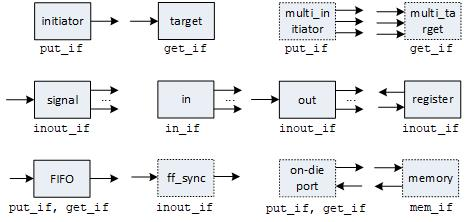
\includegraphics[width=0.9\textwidth]{pics/ss_channels.jpg}
\caption{SingleSource channels}
\label{fig:ss_channels}
\end{figure}

Target and Initiator are intended to connect two SC modules with 1:1 connection. Multi-target and Multi-initiator modules provides 1:N connection to connect multiple SC modules. FIFO is intended to connect two processes in the same module or to serve as a buffer for one process.
On-die port represents any external port to connect SC design to other IPs or fabric. Memory represents any kinds of on-chip SRAM, RF or ROM memory. Register is used to add state for METHOD process. The common use cases of the modules are given in the picture below.

Multi-initiator, multi-target, FF synchronizer, on-die port, and memory are not open-sourced yet.

\begin{figure}[!htb]
\centering
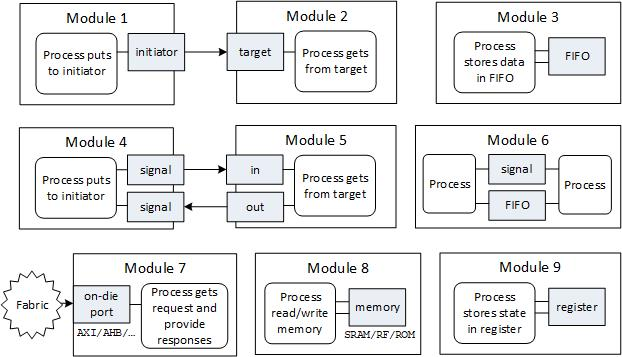
\includegraphics[width=0.9\textwidth]{pics/ss_usage.jpg}
\caption{SingleSource channels usage}
\label{fig:ss_usage}
\end{figure}

The Single Source modules work in two modes: cycle accurate (RTL) and approximate time (TLM). Cycle accurate (RTL) mode intended for hardware synthesis. In RTL mode the modules provide cycle accurate simulation. Approximate time (TLM, Transaction Level Modeling) mode provide fast simulation, intended for virtual prototyping. In TLM mode the modules provide approximate time simulation, there is no clock. Simulation is request-driven, executed in ordered delta-cycles (DC).

\subsubsection{Library files}

\begin{itemize}
\item sct\_common.h -- includes of all library headers and adds namespace \textbf{sct}
\item sct\_ipc\_if.h -- interfaces, general template types and defines
\item sct\_initiator.h -- initiator module
\item sct\_target.h -- target and combinational target modules
\item sct\_multi\_initiator.h -- initiator to connect multiple targets
\item sct\_multi\_target.h -- target to connect multiple initiators
\item sct\_prim\_signal.h -- primitive channel signal implementation with multiple drivers support
\item sct\_signal.h -- signal implementation
\item sct\_ports.h -- input and output ports, sc\_port for target and initiator
\item sct\_fifo.h -- FIFO module
\item sct\_prim\_fifo.h -- primitive channel FIFO implementation, used as base channel in TLM mode
\item sct\_register.h -- register to store METHOD state
\item sct\_clock.h -- clock with enable/disable
\item sct\_clk\_gate\_cell.h -- clock gate and clock gate signal
\item sct\_ff\_sync\_cell.h -- Flip-Flop synchronizer
\item sct\_ff\_sync\_cell.sv -- Flip-Flop synchronizer RTL implementation
\end{itemize}

\subsubsection{Library defines}
{\tt SCT\_TLM\_MODE} could be provided as compile definition: if {\tt SCT\_TLM\_MODE} defined TLM mode is used, RTL mode is used otherwise.

There are multiple options for clock/reset levels:

\begin{itemize}
\item {\tt SCT\_CMN\_TRAITS} -- clock edge and reset level, one of six following options:
\item {\tt SCT\_POSEDGE\_NEGRESET} -- positive clock edge, negative reset level
\item {\tt SCT\_POSEDGE\_POSRESET} -- positive clock edge, positive reset level
\item {\tt SCT\_NEGEDGE\_NEGRESET} -- negative clock edge, negative reset level
\item {\tt SCT\_NEGEDGE\_POSRESET} -- negative clock edge, positive reset level
\item {\tt SCT\_BOTHEDGE\_NEGRESET} -- both clock edges, negative reset level
\item {\tt SCT\_BOTHEDGE\_POSRESE}T -- both clock edges, positive reset level
\end{itemize}

Usually, positive clock edge and negative reset level are used. That is provided by define {\tt  SCT\_CMN\_TRAITS}:
\begin{lstlisting}[style=mycpp]
#ifndef SCT_CMN_TRAITS
  #define SCT_CMN_TRAITS SCT_POSEDGE_NEGRESET
#endif
\end{lstlisting}

If other clock edge/reset levels required, {\tt SCT\_CMN\_TRAITS} value should be provided as compile definition.

There is an {\tt CMakeLists.txt} example where {\tt sct\_def\_traits} target has definitions for TLM mode, negative clock edge and positive reset level:
\begin{lstlisting}[style=mycmake]
add_executable(sct_def_traits sc_main.cpp)
target_compile_definitions(sct_def_traits PUBLIC -DSCT_TLM_MODE)
target_compile_definitions(sct_def_traits PUBLIC -DSCT_CMN_TRAITS=SCT_NEGEDGE_POSRESET)
\end{lstlisting}


\subsection{Library interfaces}\label{section:sct_interfaces}

The interfaces contain non-blocking functions except {\tt b\_put} and {\tt b\_get} which are may-blocking.

Interface {\tt sct\_put\_if}:
\begin{itemize}
\item {\tt bool ready()} -- Return true if it is ready to put request,
\item {\tt void reset\_put()} -- Reset this initiator/FIFO, 
\item {\tt void clear\_put()} -- Clear (remove) request put in this cycle,
\item {\tt bool put(const T\& data)} -- Non-blocking put request into initiator/FIFO if it is ready, return ready to request, 
\item {\tt bool put(const T\& data, sc\_uint<N> mask)} -- Non-blocking put request into initiator/FIFO if it is ready, mask  used to enable/disable put or choose targets in multi-cast put, return ready to request, 
\item {\tt void b\_put(const T\& data)} -- May-blocking put request, could be used in THREAD process only,
\item {\tt void addTo(sc\_sensitive\& s)} -- Add put related signals to process sensitivity,
\item {\tt void addTo(sc\_sensitive* s, sc\_process\_handle* p)} -- Add put related signals to process sensitivity.
\end{itemize}

Interface {\tt sct\_get\_if}:
\begin{itemize}
\item {\tt bool request()} -- Return true if it has request to get,
\item {\tt void reset\_get()} -- Reset this target/FIFO,
\item {\tt void clear\_get()} -- Clear (return back) request got in this cycle,
\item {\tt T peek()} -- Peek request, return current request data, if no request last data returned,
\item {\tt T get()} -- Non-blocking get request and remove it from FIFO/target, return current request data, if no request last data returned,
\item {\tt bool get(T\& data, bool enable)} -- Non-blocking get request and remove it from FIFO/target if {\tt enable} is true, return true if there is a request and {\tt enable} is true,
\item {\tt T b\_get()} -- May-blocking get request, could be used in THREAD process only,
\item {\tt void addTo(sc\_sensitive\& s)} -- Add get related signals to process sensitivity,
\item {\tt void addTo(sc\_sensitive* s, sc\_process\_handle* p)} -- Add get related signals to process sensitivity,
\item {\tt void addPeekTo(sc\_sensitive\& s)} -- Add peek related signal to process sensitivity.
\end{itemize}

Interface {\tt sct\_fifo\_if} inherits sct\_put\_if<T> and sct\_get\_if<T> and has the following additional functions:
\begin{itemize}
\item {\tt unsigned size()} -- FIFO size,
\item {\tt unsigned elem\_num()} -- Number of elements in FIFO, value updated last clock edge for METHOD, last DC for THREAD,
\item {\tt bool almost\_full(const unsigned\& N)} -- Return true if FIFO has (LENGTH-N) elements or more, value updated last clock edge for METHOD, last DC for THREAD,
\item {\tt void clk\_nrst(sc\_in<bool>\& clk\_in, sc\_in<bool>\& nrst\_in)} -- Bind clock and reset to FIFO,
\item {\tt void addTo(sc\_sensitive\& s}) -- Add put and get related signal to process sensitivity,
\item {\tt void addToPut(sc\_sensitive\& s)} -- Add put related signals to process sensitivity,
\item {\tt void addToGet(sc\_sensitive\& s)} -- Add get related signals to process sensitivity.
\end{itemize}

Interface {\tt sct\_in\_if}:
\begin{itemize}
\item {\tt const T\& read()} -- Read from signal/register,
\item {\tt void addTo(sc\_sensitive* s, sc\_process\_handle* p)} -- Add signals to process sensitivity.
\end{itemize}

Interface {\tt sct\_inout\_if}:
\begin{itemize}
\item {\tt const T\& read()} -- Read from signal/register,
\item {\tt void write(const T\& val)} -- Write to signal/register,
\item {\tt void addTo(sc\_sensitive* s, sc\_process\_handle* p)} -- Add signals to process sensitivity.
\end{itemize}

Functions addTo, addToPut, addToGet and addPeekTo are used to add the channel to process sensitivity list. For target and initiator instead addTo {\tt operator <<} can be used. For FIFO instead addToPut and addToGet operator {\tt << fifo.PUT}, {\tt << fifo.GET}, and {\tt << fifo.PEEK} can be used.

\subsection{Processes}\label{section:sct_processes}

SystemC design with single source library can use method and thread processes created with {\tt SC\_METHOD} and {\tt SC\_THREAD} correspondently. It is recommended to use {\tt SCT\_METHOD} and {\tt SCT\_THREAD} macros instead them. Clocked thread process created with {\tt SC\_CTHREAD} is normally not used.

All the channels used in a thread process should use the same clock and edge as the process sensitive. A channel could have different reset or reset level than thread process. If all the channels have different reset or reset level, process reset is specified with third parameter of {\tt SCT\_THREAD} macro.

If a thread process has reset signal, it should have the reset specification with {\tt async\_reset\_signal\_is} or/and {\tt sync\_reset\_signal\_is}. A thread process should be sensitive to all single source channels accessed in its function code. If process is sensitive only to signal and input/output ports, the clock is provided with second parameter of {\tt SCT\_THREAD} macro.

Method process should be sensitive to all single source channels accessed in its function code. Method should not be sensitive to reset, as its provided implicitly through the channels used.

\begin{lstlisting}[style=mycpp]
template <class T>
class MyModule : public sc_module {
   sc_in<bool>      clk{"clk"};
   sct_target<T>    targ{"targ"};
   sct_initiator<T> init{"init"};
   sct_signal<T>    s{"s"};

   explicit MyModule(const sc_module_name& name) : sc_module(name) {
        SC_THREAD(thrdProc1); 
        sensitive << targ;                     // Clock and reset taken from targ
        async_reset_signal_is(nrst, 0);        // Reset specification required

        SCT_THREAD(thrdProc2, clk, nrst);      // Clock and reset explicitly provided
        sensitive << s;
        async_reset_signal_is(nrst, 0);        // Reset specification required 

        SC_METHOD(methProc); 
        sensitive << init;                     // No reset in sensitivity
   }
};
\end{lstlisting}

If any process sensitive to a channel which is not read inside or not sensitive to a channel which is read inside, error reported by ICSC. The error is reported for single channels and for vector/array of channels, no individual channels in vector/array are considered here.


\subsection{Target and Initiator}\label{section:sct_targ_init}

Target and Initiator are channels intended to connect two user defined modules. Initiator implements {\tt sct\_put\_if} interface and could be used in one METHOD or THREAD process to put requests. Target implements {\tt sct\_get\_if} interface and could be used in one METHOD or THREAD process to get requests which put by the connected Initiator.

To connect two modules, Target placed in one modules, Initiator in another one. Target and Initiator should be connected to clock and reset with {\tt clk\_nrst()} function. Target and Initiator are connected to each other with method {\tt bind()}, called in their common parent module constructor. Both Target and Initiator have method {\tt bind()}, any of them can be called.

\begin{figure}[!htb]
\centering
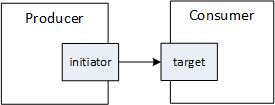
\includegraphics[width=0.5\textwidth]{pics/ss_targ_init.jpg}
\caption{Target and Initiator channels}
\label{fig:ss_usage}
\end{figure}

\begin{lstlisting}[style=mycpp]
struct Producer : public sc_module {
    sc_in<bool>         clk{"clk"};
    sc_in<bool>         nrst{"nrst"};
    sct_initiator<T>    init{"init"};
    explicit Producer (const sc_module_name& name) : sc_module(name) {
        init.clk_nrst(clk, nrst);
    } 
}
struct Consumer : public sc_module {
    sc_in<bool>         clk{"clk"};
    sc_in<bool>         nrst{"nrst"};
    sct_target<T>       targ{"targ"};
    explicit Consumer (const sc_module_name& name) : sc_module(name) {
        targ.clk_nrst(clk, nrst);
    } 
}
struct Top: public sc_module {
    Producer prod{"prod"};
    Consumer cons{"cons"};
    explicit Top(const sc_module_name& name) : sc_module(name) {
        prod.clk(clk); prod.nrst(nrst);
        cons.clk(clk); cons.nrst(nrst);
        // Call bind() method of initiator or bind() method of target
        prod.init.bind(cons.targ);  
    }
}
\end{lstlisting}

Target and Initiator have the same template parameters:
\begin{lstlisting}[style=mycpp]
template<
    class T,                              // Payload data type 
    class TRAITS = SCT_CMN_TRAITS,        // Clock edge and reset level traits
    bool TLM_MODE = SCT_CMN_TLM_MODE>     // RTL (0) or TLM (1) mode
class sct_initiator {};

template<
    class T,                              // Payload data type 
    class TRAITS = SCT_CMN_TRAITS,        // Clock edge and reset level traits
    bool TLM_MODE = SCT_CMN_TLM_MODE>     // RTL (0) or TLM (1) mode
class sct_target {};
\end{lstlisting}

Target and Initiator constructor parameters:
\begin{lstlisting}[style=mycpp]
sct_target(const sc_module_name& name, 
           bool sync_ = 0,                // Is register required to pipeline request 
           bool always_ready_ = 0);       // Is always ready to get request

sct_initiator(const sc_module_name& name,
           bool sync_ = 0);               // Is register required to pipeline request  
\end{lstlisting}

\subsection{Target and initiator usage}\label{section:sct_targ_init_usage}

Target and initiator can be used in SystemC method process. The method process should be created with {\tt SC\_METHOD} or {\tt SCT\_METHOD}  macro in the module constructor. The method process should have sensitivity list with all the targets/initiators accessed in the process function.

\begin{lstlisting}[style=mycpp]
// Initiator and target in method process example
struct Producer : public sc_module {
    sct_initiator<T>         init{"init"};
    explicit Producer (const sc_module_name& name) : sc_module(name) {
       SC_METHOD(initProc); 
       sensitive << init;
    } 
    void initProc {
       // Put data into init
    }
}

struct Consumer : public sc_module {
    sct_target<T>       targ{"targ"};   
    explicit Consumer (const sc_module_name& name) : sc_module(name) {
       SC_METHOD(targProc); 
       sensitive << targ;
    } 
    void targProc{
       // Get data from targ
    }
}
\end{lstlisting}

Target and initiator can be used in clocked thread process. Clocked thread process should be created with {\tt SC\_THREAD} or {\tt SCT\_THREAD} macro, but not with {\tt SC\_CTHREAD}. The thread process should have sensitivity list with all the targets/initiators accessed in the process function as for method process. If the thread process has reset signal, it should have the reset specification with {\tt async\_reset\_signal\_is} or/and {\tt sync\_reset\_signal\_is}.

\begin{lstlisting}[style=mycpp]
// Initiator and target in thread process example
struct Producer : public sc_module {
    sct_initiator<T>         init{"init"};
    explicit Producer (const sc_module_name& name) : sc_module(name) {
       SC_THREAD(initProc); 
       sensitive << init;
       async_reset_signal_is(nrst, 0);
    } 
    void initProc {
       // Reset init to set default values
       wait();
       while(true) {
          // Put data into init 
          wait();
       }
    }
}

struct Consumer : public sc_module {
    sct_target<T>       targ{"targ"};   
    explicit Consumer (const sc_module_name& name) : sc_module(name) {
       SC_THREAD(targProc); 
       sensitive << targ;
       async_reset_signal_is(nrst, 0);
    } 
    void targProc{
       // Reset init to set default values
       wait();
       while(true) {
          // Get data from targ
          wait();
       }
    }
}
\end{lstlisting}

There are three kinds of connections which could be organized:
\begin{itemize}
\item Combinational,
\item Buffered,
\item Buffered with FIFO.
\end{itemize}

\subsubsection{Combinational connection}

In combinational connection request part of connection contains {\tt core\_req} and {\tt core\_data} signals, which could be used directly or through the pipelining register (specified with second parameter of Target/Initiator constructor). There is no back-pressure signal, so Target process should be always ready to get request. Initiator process does not need to check ready to put request (method {\tt ready()} always returns true).

\begin{figure}[!htb]
\centering
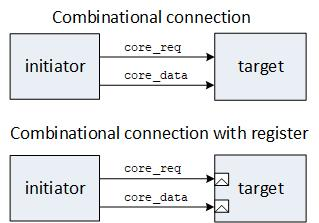
\includegraphics[width=0.5\textwidth]{pics/ss_comb_conn.jpg}
\caption{Combinational connection}
\label{fig:ss_usage}
\end{figure}

Combinational connection is provided with last parameter of {\tt sct\_target<>} constructor or with using special target class {\tt sct\_comb\_target<>}.

In combinational connection put data into Initiator can be done without checking if the Initiator is ready.

\begin{lstlisting}[style=mycpp]
// Initiator and always ready target in method process example
struct Producer : public sc_module {
    sct_initiator<T>         init{"init"};
    explicit Producer (const sc_module_name& name) : sc_module(name) {
       SC_METHOD(initProc); sensitive << init;
    } 
    void initProc {
       T val = getSomeValue();          // Put at every path, reset is not required 
       init.put(val);                   // Do not check ready() as Target is always ready
    }						   
}

struct Consumer : public sc_module {
    // Combinational target
    sct_comb_target<T>       targ{"targ"};   
    explicit Consumer (const sc_module_name& name) : sc_module(name) {
       SC_METHOD(targProc); sensitive << targ;
    } 
    void targProc{
       T val;
       if (targ.get(val)) {             // Get at every path, reset is not required
           doSomething(val);        
       }
    }
}
\end{lstlisting}

In thread process it needs to reset Initiator and Target in the reset section.
\begin{lstlisting}[style=mycpp]
// Initiator and always ready target in thread process example
struct Producer : public sc_module {
    sct_initiator<T>         init{"init"};
    explicit Producer (const sc_module_name& name) : sc_module(name) {
       SC_THREAD(initProc); sensitive << init;
       async_reset_signal_is(nrst, 0);
    } 
    void initProc {
       init.reset_put();                 // Reset is required in thread process
       wait();
       while(true) {
          T val = getSomeValue();        // Put every cycle
          init.put(val);                 // Do not check ready() as Target is always ready
          wait();				   
       }
    }
}

struct Consumer : public sc_module {
    sct_comb_target<T>       targ{"targ"};   
    explicit Consumer (const sc_module_name& name) : sc_module(name) {
       SC_THREAD(targProc); sensitive << targ;
       async_reset_signal_is(nrst, 0);
    } 
    void targProc{
       targ.reset_get();                 // Reset is required in thread process
       wait();
       while(true) {
          if (targ.request()) {         
              doSomething(targ.get());
          }
          wait();
       }
    }
}
\end{lstlisting}
Using Target and Initiator in method and thread process looks very similar. In the next sections examples using method and thread process will be mixed.

\subsubsection{Buffered connection}

In buffered connection {\tt core\_ready} signal is used as backpressure when Target is not ready to get request. This connection called buffered as it has the buffer register inside Target or Initiator to store one request if Target is not ready. This kind of connection is the most common and used as default one.

Request part of the connection contains {\tt core\_req} and {\tt core\_data} signals, which could be used directly or through the pipelining register (specified with second parameter of Target/Initiator constructor). The pipelining register is additional to the buffer register. Response part contains {\tt core\_ready} signal which is passed through register to avoid combinational loop. If target process is method this register explicitly added, if it is thread this register is implicitly provided by the process.

\begin{figure}[!htb]
\centering
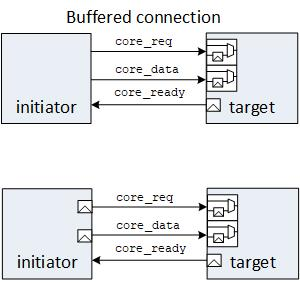
\includegraphics[width=0.5\textwidth]{pics/ss_buff_conn.jpg}
\caption{Buffered connection}
\label{fig:ss_usage}
\end{figure}

\begin{lstlisting}[style=mycpp]
struct Producer : public sc_module {
    sct_initiator<T>         init{"init"};
    explicit Producer (const sc_module_name& name) : sc_module(name) {
       SC_METHOD(initProc); sensitive << init;
    } 
    void initProc {
       init.reset_put();                  // Reset required as put done at some paths only  
       if (init.ready()) {                // Check ready required, target can be not ready 
          init.put(getSomeValue());
       }
    }
}

struct Consumer : public sc_module {
    sct_target<T>       targ{"targ"};
    explicit Consumer (const sc_module_name& name) : sc_module(name) {
       SC_THREAD(targProc); sensitive << targ;
       async_reset_signal_is(nrst, 0);
    } 
    void targProc {
       targ.reset_get();
       wait();
       while(true) {
          if (targ.request()) {      
              doSomething(targ.get()); 
          }
          wait(); 
       }
    }
}
\end{lstlisting}


\subsubsection{Buffered connection with FIFO}

The buffered connection with FIFO provides additional buffer to store requests until their processed by the target process. FIFO can be added to Target with {\tt add\_fifo()} method:

\begin{lstlisting}[style=mycpp]
template<unsigned LENGTH>                  // FIFO size (maximal number of elements)
void add_fifo(bool sync_valid = 0,         // Is register required to pipeline request
          bool sync_ready = 0,             // Is register required to pipeline ready 
          bool init_buffer = 0);           // Initialize all the elements with zeros 
                                           // First element to get is always initialized
\end{lstlisting}

\begin{figure}[!htb]
\centering
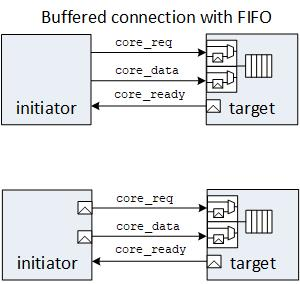
\includegraphics[width=0.5\textwidth]{pics/ss_buff_fifo_conn.jpg}
\caption{Buffered connection with FIFO}
\label{fig:ss_usage}
\end{figure}

\begin{lstlisting}[style=mycpp]
template<class T>
struct A : public sc_module {
    sct_target<T>       run{"run"}; 
    explicit A(const sc_module_name& name) : sc_module(name) {
        run.clk_nrst(clk, nrst);
        run.template add_fifo<2>(1, 1);  // Add FIFO with 2 element and registers 
    }
}
\end{lstlisting}

\subsubsection{Initiator-to-Target Protocol}

The discussed protocol considers buffered connection w/o FIFO. Request is taken by Target when {\tt core\_req} and {\tt core\_ready} both are high. Target can return it to the target process immediately or store the request in the buffer. Initiator sets new request when the previous one has been taken.

The first diagram below represents Target and Initiators accessed in thread processes. The second diagram represents Target and Initiators accessed in method processes.

\begin{figure}[!htb]
\centering
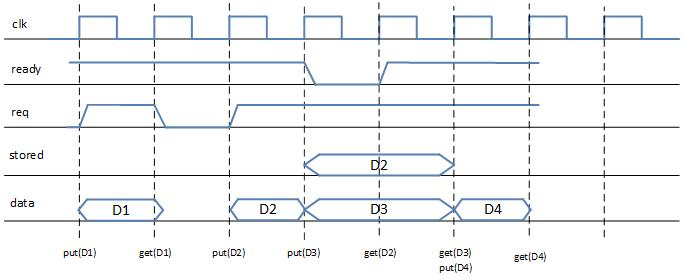
\includegraphics[width=0.98\textwidth]{pics/ss_prot_tt.jpg}
\caption{Initiator-to-Target in THREAD processes}
\label{fig:ss_usage}
\end{figure}

\begin{figure}[!htb]
\centering
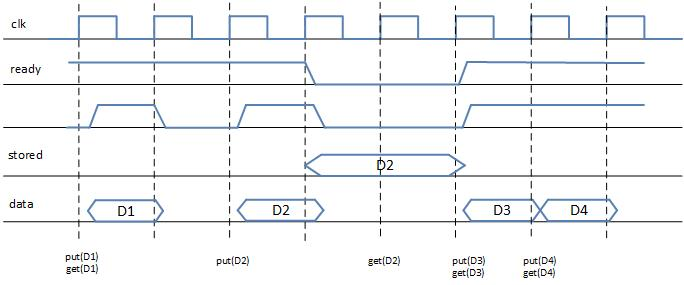
\includegraphics[width=0.98\textwidth]{pics/ss_prot_mm.jpg}
\caption{Initiator-to-Target in METHOD processes}
\label{fig:ss_usage}
\end{figure}

\subsection{Signal and ports}\label{section:sct_signal}
Signal can be used for inter-process communication between processes in the same module. For communication between processes in different modules input/output ports are used together with signal.

\begin{figure}[!htb]
\centering
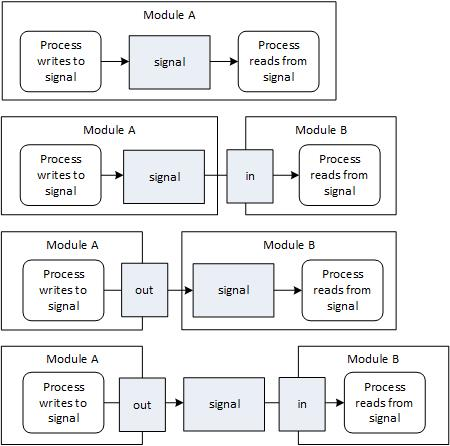
\includegraphics[width=0.7\textwidth]{pics/ss_sig_usage.jpg}
\caption{Signal and ports}
\label{fig:ss_usage}
\end{figure}

Signal and output port implement {\tt sct\_inout\_if}, and can be written by one process. Signal, input and output ports implement {\tt sct\_in\_if}, and can be read by one or mode processes.

\begin{lstlisting}[style=mycpp]
template<
    class T, bool TLM_MODE = SCT_CMN_TLM_MODE>
class sct_signal {};
template<
    class T, bool TLM_MODE = SCT_CMN_TLM_MODE>
class sct_in {};
template<
    class T, bool TLM_MODE = SCT_CMN_TLM_MODE>
class sct_out {};
\end{lstlisting}

Using signal and input/output ports in thread process requires to have clock/reset for these channels which provided with {\tt SCT\_THREAD} macro:
\begin{lstlisting}[style=mycpp]
// Used if the process sensitive to signals/ports only  
SCT_THREAD(proc, clk, rst);  
// Used if the process sensitive to signals/ports and other channels
SCT_THREAD(proc, clk);       
\end{lstlisting}

In this example sigThread sensitive to signals only:
\begin{lstlisting}[style=mycpp]
sct_signal<T>   s{"s"};
MyModule(const sc_module_name& name) : sc_module(name) {  
   // Clock edge/reset level taken from SCT_CMN_TRAITS
   SCT_THREAD(sigThread, clk, nrst); 
   // Only signal `s` is read inside the process
   sensitive << s;                   
   async_reset_signal_is(nrst, 0);
}
\end{lstlisting}

{\tt sc\_vector} of {\tt sct\_signal}, {\tt sct\_in} and {\tt sct\_out} supported. Binding of while vector to another vector is supported.
\begin{lstlisting}[style=mycpp]
class A : public sc_module {
    sc_vector<sct_out<T>>      resp{"resp", 3};
};
class Top {
    A   a{"a"};
    sc_vector<sct_signal<T>>   resp{"resp", 3};

    Top (const sc_module_name& name) : sc_module(name) {        
        a.resp(resp);                  // All vector elements bound
    }
}
\end{lstlisting}

In RTL mode {\tt sct\_signal} is based on {\tt sc\_signal}, {\tt sct\_in}/{\tt sct\_out} are based on {\tt sc\_in}/{\tt sc\_out}.


\subsection{FIFO}\label{section:sct_fifo}

The FIFO can be used for inter-process communication between processes in the same module and for storing requests inside one process. Also the FIFO could be used inside of Target as an extended buffer.

\begin{figure}[!htb]
\centering
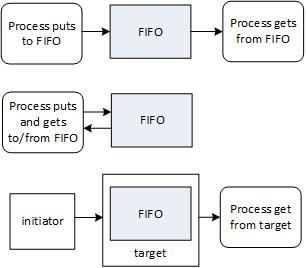
\includegraphics[width=0.5\textwidth]{pics/ss_fifo.jpg}
\caption{FIFO}
\label{fig:ss_fifo}
\end{figure}

FIFO implements {\tt sct\_fifo\_if} interface. FIFO has size template parameter which is a positive number.
\begin{lstlisting}[style=mycpp]
template<
    class T, 
    unsigned LENGTH,                      // Size (maximal number of elements)
    class TRAITS = SCT_CMN_TRAITS,        // Clock edge and reset level traits
    bool TLM_MODE = SCT_CMN_TLM_MODE>     // RTL (0) or TLM (1) mode
>
class sct_fifo {};
\end{lstlisting}

FIFO can have combinational or registered request ({\tt core\_req} and {\tt core\_data}) and response ({\tt core\_ready}) kind which specified in constructor parameters.
\begin{lstlisting}[style=mycpp]
sct_fifo(const sc_module_name& name, 
         bool sync_valid = 0,            // Request path has synchronous register 
         bool sync_ready = 0,            // Response path has synchronous register  
         bool use_elem_num = 0,          // Element number/Almost full or empty used 
         bool init_buffer = 0)           // Initialize all buffer elements with zeros in reset
                                         // First element to get is always initialized to zero 
\end{lstlisting}

\subsubsection{Minimal FIFO size required}

Minimal FIFO size required given in Table.~\ref{tab:fifo_size}.
\begin{table}
\begin{tabular}{|l|l|l|l|l|}
\hline
Initiator process & Target process & sync\_valid & sync\_ready & Minimal FIFO size \\
\hline
method & method & 0 & 0 & 1 \\
method & method & 0 & 1 & 1 \\
method & method & 1 & 0 & 1 \\
method & method & 1 & 1 & 2 \\
method & thread & 0 & 0 & 1 \\
method & thread & 0 & 1 & 2 \\
method & thread & 1 & 0 & 2 \\
method & thread & 1 & 1 & 3 \\
thread & method & 0 & 0 & 1 \\
thread & method & 0 & 1 & 2 \\
thread & method & 1 & 0 & 2 \\
thread & method & 1 & 1 & 3 \\
thread & thread & 0 & 0 & 2 \\
thread & thread & 0 & 1 & 3 \\
thread & thread & 1 & 0 & 3 \\
thread & thread & 1 & 1 & 4 \\
\hline
\end{tabular}
\caption{Minimal FIFO size}
\label{tab:fifo_size}
\end{table}

\subsubsection{Using FIFO for inter-process communication}

FIFO could be used for processes communication instead of set of signals. FIFO has only one writer and one reader process, in comparison with {\tt sct\_signal} which could be read in multiple processes. For 1:N communication array or {\tt sc\_vector} of FIFOs could be used.

\begin{lstlisting}[style=mycpp]
struct Top : public sc_module {
    sct_fifo<T, 2>      fifo{"fifo", 1};     // Pipelining register for request
    explicit Top(const sc_module_name& name) : sc_module(name) {
        fifo.clk_nrst(clk, nrst);
        SC_THREAD(producerProc); 
        sensitive << fifo.PUT;               // Process puts to FIFO
        async_reset_signal_is(nrst, 0);
        SC_METHOD(consumerProc); 
        sensitive << fifo.GET;               // Process gets from FIFO   
    } 
}

void producerProc() {
    fifo.reset_put();
    wait();
    while (true) {
       if (fifo.ready()) {                  // If FIFO is ready put next value
          fifo.put(getSomeVal());
       }
       wait();
    }
}
void consumerProc() {
    fifo.reset_get();
    T val;
    if (fifo.get(val)) {
       doSomething(val);
    }
}
\end{lstlisting}

\subsubsection{One process stores requests in FIFO}

One process stores requests in FIFO example.
\begin{lstlisting}[style=mycpp]
struct Top : public sc_module {
    sc_in<bool>         clk{"clk"};
    sc_in<bool>         nrst{"nrst"};
    sct_fifo<T, 5>      fifo{"fifo"};
    explicit Top(const sc_module_name& name) : sc_module(name) {
        fifo.clk_nrst(clk, nrst);
        SC_THREAD(storeProc); 
        sensitive << fifo;                 // Process puts and gets to FIFO
        async_reset_signal_is(nrst, 0);
    }
}

void storeProc() {
    fifo.reset();
    wait();
    while (true) {
       if (fifo.ready()) {
          fifo.put(getSomeValue());
       }
       wait(); 
       if (fifo.request()) {
          doSomething(fifo.get());
       }
    }
}
\end{lstlisting}


\subsection{Register}

Register is used to add state for METHOD process. Register is written in one method process and could be read in the same or other method process(es). Register is normally added to sensitivity list of process where it is read. Register can be read in thread process.

\begin{figure}[!htb]
\centering
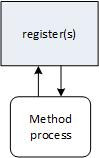
\includegraphics[width=0.17\textwidth]{pics/ss_reg.jpg}
\caption{Register}
\label{fig:ss_reg}
\end{figure}

Register has the same template parameters as Target/Initiator:
\begin{lstlisting}[style=mycpp]
template<
    class T,                            // Payload data type 
    class TRAITS = SCT_CMN_TRAITS,      // Clock edge and reset level traits
    bool TLM_MODE = SCT_CMN_TLM_MODE>   // RTL (0) or TLM (1) mode
class sct_register {};
\end{lstlisting}

Register has the following methods:

\begin{lstlisting}[style=mycpp]
// Reset register, set it value to stored at last clock edge
void reset();
// Write new value to register
void write(const T& data);
// Read value stored at last clock edge
T read();
// To skip using read()
operator T ();
\end{lstlisting}

Register can initiate a new request. That means an output request can depend on register state.

\begin{lstlisting}[style=mycpp]
sct_target<T>       targ{"targ"};
sct_register<T>     cntr{"cntr"};
explicit A(const sc_module_name& name) : sc_module(name) {
    targ.clk_nrst(clk, nrst);
    cntr.clk_nrst(clk, nrst);
    SC_METHOD(checkProc); sensitive << targ << cntr;
}

void checkProc() {
    cntr.reset();
    // Register accumulates received data up to N
    if (cntr.read() > N) {
        cntr.write(0); 
    } else 
    if (targ.get(data)) {
        cntr.write(cntr.read()+data); 
    }
}
\end{lstlisting}


Read register in thread process should be done carefully. If register value is checked to generate an output or change a state, it could lead to incorrect behavior in TLM, if there is no other activation source for the process. 
\begin{lstlisting}[style=mycpp]
sct_register<T>     cntr{"cntr"};
sct_initiator<T>    init{"init"};
explicit A(const sc_module_name& name) : sc_module(name) {
    cntr.clk_nrst(clk, nrst);
    init.clk_nrst(clk, nrst);
    SCT_THREAD(cntrProc); sensitive << cntr << init;
    async_reset_signal_is(nrst, 0);
    // cntr is assigned in some method process 
}

// Probably incorrect version
void cntrProc() {
    init.reset_put();
    wait();
    while (true) {
        if (cntr.read() > 10) {          // In TLM mode no process activation 
           init.b_put(cntr.read());      // until cntr value changed
        }
        wait();
    }
}

// Correct version
void cntrProc() {
    init.reset_put();
    T lastCntr = 0;
    wait();
    while (true) {
        // Request sent only when cntr value changed  
        if (cntr.read() > 10 && cntr.read() != lastCntr) {
           lastCntr = cntr.read();       
           init.b_put(cntr.read());     
        }
        wait();
    }
}
\end{lstlisting}
The same problem is actual for {\tt sct\_signal}.

\subsection{Clock, clock gate and clock gate signal}

{\tt sct\_clock<>} is implementation of clock source (generator) like {\tt sc\_clock} with enable/disable control.

\begin{lstlisting}[style=mycpp]
    /// Enable clock activity, clock is enabled after construction 
    void enable();   
    /// Disable clock activity, can be called at elaboration phase to disable
    /// clock at simulation phase start
    void disable();    
    /// Register clock gate signals/ports to control clock activity.
    /// If any of the signals/ports is high, then clock is enabled
    void register_cg_enable(sc_signal_inout_if<bool>& enable);
    /// Get clock period    
    const sc_time& period() const;
\end{lstlisting}

Clock gate cell {\tt sct\_clock\_gate\_cell} and clock signal {\tt sct\_clk\_signal} should be used together to connect clock input to gated clock source. {\tt sct\_clk\_signal} is special signal without DC delay in written value becomes readable.

\begin{figure}[!htb]
\centering
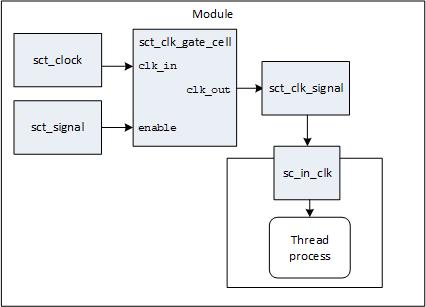
\includegraphics[width=0.7\textwidth]{pics/ss_clock.jpg}
\caption{Clock and clock gate}
\label{fig:ss_clock}
\end{figure}

The code example illustrates using  {\tt sct\_clock\_gate\_cell} and  {\tt sct\_clk\_signal}.

\begin{lstlisting}[style=mycpp]
SC_MODULE(A) {
    sc_in_clk               SC_NAMED(clk);
    sc_in<bool>             SC_NAMED(nrst); 
    sc_in<bool>             SC_NAMED(clk_enbl);
    sct_clk_signal          SC_NAMED(clk_out);
    sct::sct_clk_gate_cell  SC_NAMED(clk_gate);
    sc_in<bool>             SC_NAMED(clk_in);

    explicit A(const sc_module_name& name) : sc_module(name) {
        clk_gate.clk_in(clk);        // Clock input
        clk_gate.enable(clk_enbl);   // Gate clock input 
        clk_gate.clk_out(clk_out);   // Gated clock output    
        clk_in(clk_out);
        
        SCT_THREAD(thrdProc, clk_in, nrst);   // Use clock input bound to gated clock
        async_reset_signal_is(nrst1, 0);
}};
\end{lstlisting}

Clock gate cells can be sequentially connected to each other, gated clock output of one cell bound to clock input of anther cell.

In TLM mode is all thread processes are created with {\tt SC\_THREAD}/{\tt SCT\_THREAD} macros, clock source(s) can be disabled. Disabling {\tt sct\_clock} allows to speed simulation:
\begin{lstlisting}[style=mycpp]
sct_clock<>     clk{"clk", 1, SC_NS};
explicit A(const sc_module_name& name) : sc_module(name) {
    if (SCT_CMN_TLM_MODE) {
         clk.disable();
    }
}
\end{lstlisting}

\subsection{Reset}

\subsubsection{Reset section}

In thread process reset logic initializes registers, local variables and output signals. This logic should be placed in reset section (code scope before first {\tt wait()}).
\begin{lstlisting}[style=mycpp]
sct_out<T> o{"o"};
sct_signal<T> s{"s"};
void thrdProc() {
    // Reset section
    int a = 0;                  // Local variable
    s = 0;                      // Register 
    o = 0;                      // Output 
    wait();
    while (true) {
        ...
        wait(); 
    } 
}
\end{lstlisting}

In method process initialization logic initializes local variables and output signals. This logic is normally be placed in the beginning of the process.
\begin{lstlisting}[style=mycpp]
sct_out<T> o{"o"};
void methdProc() {
    // Initialization section
    int a = 0;                  // Local variable
    o = 0;                      // Output 
    ...
    a = i + 1;
    if (s) o = a;
}
\end{lstlisting}

Initialization logic in method process could be merged with its behavior logic based on inputs and registers. Such code style can have better simulation performance.
\begin{lstlisting}[style=mycpp]
sct_in<T> i{"i"};
sct_out<T> o{"o"};
void methdProc() {
    int a = i+1;                // Local variable
    o = a ? s : 0;              // Output 
    ...
}
\end{lstlisting}

The communication channels also need to be reset with specified {\tt reset()}, {\tt reset\_get()} and {\tt reset\_put()} methods. In thread process every channel used in this process should be initialized in the reset section.
\begin{lstlisting}[style=mycpp]
sct_initiator<T>  init{"init"};
sct_target<T>     targ{"targ"};
sct_fifo<T, 2>    fifo{"fifo"};
void thrdProc() {
    init.reset();
    targ.reset();
    fifo.reset_put();           // If FIFO used for put
    fifo.reset_get();           // If FIFO used for get
    fifo.reset();               // If FIFO used for get and put both
    wait();
    while (true) {
        ...
        wait(); 
    } 
}
\end{lstlisting}

In method process every channel used in this process is initialized in the beginning of the process or assigned at all execution path in the process code. Having no explicit reset for registers, signals, output ports and synchronizers can improve simulation performance.
\begin{lstlisting}[style=mycpp]
sct_initiator<T>  init{"init"};
sct_target<T>     targ{"targ"};
sct_register<T>   reg1{"reg1"};
sct_register<T>   reg2{"reg2"};
void methProc() {
    init.reset();
    reg1.reset();        
    T val = targ.get();  // targ is accessed at all path, no reset required
    if (val > 0) {
        reg1 = val;      // reg1 accessed at some paths only, reset required
        init.put(val);   // init accessed at some paths only, reset required
    }
    reg2 = val + 1;      // reg2 is accessed at all path, no reset required 
}
\end{lstlisting}


\subsubsection{Reset control}
Reset signal can be asserted/de-asserted in TB and DUT processes as well. To have the same simulation time in RTL and TLM modes it needs to follow the rules given in this section.

If reset control thread is in TB, it could control reset based on time period and be non-sensitive to any channels. In this case such a thread should be {\tt SC\_CTHREAD} in RTL mode and {\tt SC\_THREAD} in TLM mode. To avoid extra activation in TLM mode, this thread should wait for a specified time instead of clock events.
\begin{lstlisting}[style=mycpp]
SC_MODULE(A) {
   SC_CTOR(A) {
       // Thread not sensitive to anything
       #ifdef SCT_TLM_MODE
          SC_THREAD(resetProc);
       #else
          SC_CTHREAD(resetProc, clk_in.pos());
       #endif
   }
   #define rstWait(N) if (SCT_CMN_TLM_MODE) wait(N, SC_NS); else wait(N);
   void resetProc() {
        nrst = 0; 
        rstWait(3);
        cout << sc_time_stamp() << " " << sc_delta_count() << " de-assert reset\n";
        nrst = 1; 
        rstWait(5);
        ...
   } 
};
\end{lstlisting}

If reset control thread is sensitive to any channels, it should be {\tt SCT\_THREAD} and have {\tt dont\_initialize()} in RTL mode. Such a thread can also be a normal test thread which provides stimulus and checks results:
\begin{lstlisting}[style=mycpp]
SC_MODULE(A) {
   SC_CTOR(A) {
       // Thread sensitive to SS channels
        SCT_THREAD(resetProc, clk);
        #ifndef SCT_TLM_MODE
            dont_initialize();
        #endif
        sensitive << s;
   }
   sct_signal<unsigned>  s{"s"};
   void resetProc() {
        nrst = 0; 
        while (s.read() < 3) {s = s.read()+1; wait();}
        cout << sc_time_stamp() << " " << sc_delta_count() << " de-assert reset\n";
        nrst = 1; 
   }
\end{lstlisting}

\subsubsection{Specify clock edge and reset level}

Clock edge and reset level normally are the same for the design. To update them for whole design {\tt SCT\_CMN\_TRAITS} should be defined:
\begin{lstlisting}[style=mycpp]
#define SCT_CMN_TRAITS SCT_NEGEDGE_POSRESET   // Set negative edge and positive reset level
\end{lstlisting}

To specify clock edge and reset level for individual library modules, template parameters should be used, for example:
\begin{lstlisting}[style=mycpp]
sct_target<T, SCT_NEGEDGE_POSRESET>       run{"run"};
sct_initiator<T, SCT_POSEDGE_NEGRESET>    resp{"resp"};
\end{lstlisting}


\subsection{Array of SingleSource channels}

Array of SingleSource channels can be implemented with {\tt sc\_vector}. First parameter of {\tt sc\_vector} is name, second parameter is number of elements (should be a compile time constant). To provide additional parameters to single source channels, it needs to use lambda function as third parameter of {\tt sc\_vector}.

\begin{lstlisting}[style=mycpp]
static const unsigned N = 16;
using T = sc_uint<16>;
sc_vector<sct_target<T>>       targ{"targ", N};    // Two parameters 
sc_vector<sct_initiator<T>>    init{"init", N,     // Three parameters
   [](const char* name, size_t i) {                // Lambda function         
        return sc_new<sct_initiator<T>>(name, 1);  // Initiator with sync register
   }}; 
\end{lstlisting}

\subsection{Target and initiator in top module}

Target and Initiator can be instantiated in top module to be connected to the correspondent modules in testbench. Such top module is synthesizable with input/output ports for the Target/Initiator instances.

Top module can contain Target which is not always ready and has no synchronous register. Top module can contain initiator which has no synchronous register. Top module cannot contain MultiTarget or MultiInitiator. Vector ({\tt sc\_vector}) of Target/Initiator in top module is supported.

\begin{figure}[!htb]
\centering
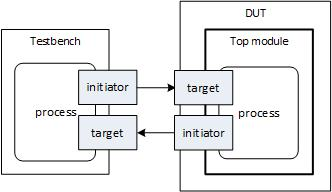
\includegraphics[width=0.55\textwidth]{pics/ss_top_mod.jpg}
\caption{Target and initiator in top module}
\label{fig:ss_top_mod}
\end{figure}

To connect testbench Target/Initiator to the correspondent top module Initiator/Target normal {\tt bind()} function is used always except multi-language simulation. For multi-language simulation if DUT is in SystemVerilog and testbench is in SystemC language, the simulation tool generates a special SystemC wrapper for DUT top module. To connect this wrapper to SystemC testbench {\tt SCT\_BIND\_CHANNEL} macro should be used. {\tt  SCT\_BIND\_CHANNEL} macro cannot be applied to Target/Initiator with record type.

\begin{lstlisting}[style=mycpp]
// Include DUT module generated wrapper or SystemC header 
#ifdef RTL_SIM
    #include "DUT.h"          // Multi-language simulation, include generated wrapper
#else 
    #include "MyDut.h"        // SystemC simulation and synthesis, include designed header
#endif

template<class T>
class MyModule : public sc_module {
   DUT                       dut{"dut"}; 
   sct_target<T>             targ{"targ"};
   SC_CTOR(MyModule) {
       // Bind targ to init in dut module 
       #ifdef RTL_SIM
           SCT_BIND_CHANNEL(dut, init, targ);         // Multi-language simulation
       #else 
           targ.bind(dut.init);                       // SystemC simulation and synthesis
       #endif
   }
}
\end{lstlisting}

\subsection{Array of Target/Initiator in top module}

Array of Targets/Initiators supported in any module including top module. Instead of C++ array {\tt sc\_vector} should be used (C++ array is not supported). To bind the Targets/Initiators {\tt SCT\_BIND\_CHANNEL} macro with 4 parameters is provided.

\begin{lstlisting}[style=mycpp]
// Include DUT module generated wrapper or SystemC header 
#ifdef RTL_SIM
    #include "DUT.h"         // Multi-language simulation, include generated wrapper
#else 
    #include "MyDut.h"       // SystemC simulation and synthesis, include designed header
#endif

template<class T, unsigned N>
class MyModule : public sc_module {
   DUT              dut{"dut"}; 
   sc_vector<sct_target<T>>    targ{"targ", N};
   SC_CTOR(MyModule) {
       // Bind all elements of targ to elements of init in dut module 
       #ifdef RTL_SIM
           SCT_BIND_CHANNEL(dut, init, targ, N);   // Multi-language simulation
       #else 
           for (unsigned i = 0; i != N; ++i)  
               targ[i].bind(dut.init[i]);          // SystemC simulation and synthesis
       #endif
   }
}
\end{lstlisting}

\subsection{Hierarchical connection of Target and Initiator}

Target and Initiator can be connected through module hierarchy from child module up to parent module. To do that {\tt sc\_port} of Initiator/Target in parent module should be used. Ports ({\tt sc\_port}) of Target/Initiator contain pointer to them. To bind Initiator to Target through ports it needs to use {\tt get\_instance()} method which provides Target/Initiator from its port.

\begin{figure}[!htb]
\centering
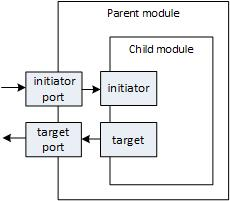
\includegraphics[width=0.4\textwidth]{pics/ss_parent_mod.jpg}
\caption{Target and initiator ports}
\label{fig:ss_parent_mod}
\end{figure}

\begin{lstlisting}[style=mycpp]
template<class T>
struct Child : public sc_module {
    sct_target<T>       run{"run"};
    sct_initiator<T>    resp{"resp"};
};

template<class T>
struct Parent: public sc_module  {
   // Target/initiator ports
    sc_port<sct_target<T>>       run;   
    sc_port<sct_initiator<T>>    resp;   

    Child<T>                     child{"child"};
  
    explicit Parent(const sc_module_name& name) : sc_module(name) {
        // Bind ports to child module target/initiator
        run(child.run);      
        resp(child.resp);
    }
};

struct Top: public sc_module  {
    Parent<T>                    parent{"parent"};
  
    explicit Parent(const sc_module_name& name) : sc_module(name) {
        // Bind child target/initiator to eahc other through parent ports
        // get_instance() provides Initiator from its sc_port   
        parent.run->bind(parent.resp->get_instance());   
    }
};
\end{lstlisting}
Process which calls Target/Initiator functions should be in the module where Target/Initiator declared. If a process calls Target/Initiator through its port ({\tt sc\_port<sct\_target>/sc\_port<sct\_initiator>}) the process module and target initiator module should be synthesized in the same parent module.

\subsection{Cycle accurate and SingleSource code mix}

Conventional cycle accurate SystemC modules can be mixed with single source modules without limitations. {\tt sct\_clock} should be used instead of normal {\tt sc\_clock}.

Cycle accurate threads created with {\tt SC\_CTHREAD} macro are activated by clock event. Such processes can use SingleSource channels to communicate to each other and SingleSource threads created with {\tt SCT\_THREAD} macro. Cycle accurate processes should be sensitive to all the SingleSource channels used inside.

\begin{lstlisting}[style=mycpp]
template<class T>
class MyModule : sc_module {
    sct_target<T>       in{"in"};
    sct_signal<T>       s{"s"};
    sct_fifo<T, 2>      fifo{"fifo"};

    MyModule(const sc_module_name& name) : sc_module(name) {
        SC_CTHREAD(threadProc, clk);
        sensitive << in << fifo.PUT << s;    // sensitivity to all used channels
        async_reset_signal_is(nrst, 0);
    }
    void threadProc() {
        in.reset_get();
        fifo.reset_put();
        wait();
        while (true) {
            if (in.request()) {
                fifo.put(s.read()); 
                in.get();
            }
            wait();
        }
    }
}
\end{lstlisting}

Instead of {\tt SC\_CTHREAD} special {\tt SCT\_CTHREAD} macro could be used. {\tt SCT\_CTHREAD} supports clock edge with third parameter:

\begin{lstlisting}[style=mycpp]
SCT_CTHREAD(proc, clk, clk_edge);   // clk_edge 0 -- negedge, 1 -- posedge, 2 -- both edges
SCT_CTHREAD(proc, clk);             // clk_edge is SCT_CMN_TRAITS::CLOCK
\end{lstlisting}

\subsection{Record as data type in SingleSource channels}

Record is supported as data type in all SingleSource channels. The record should comply SystemC requirements for records used in signal/port: the record should have default constructor w/o parameters, {\tt operator==()}, {\tt operator<<(std::ostream)} and {\tt sc\_trace()} implemented.

\begin{lstlisting}[style=mycpp]
struct Rec_t {
    bool enable;
    sc_uint<16> addr;
    // Default constructor
    Rec_t() : enable(false), addr(0) {}
    // Another constructor, optional
    Rec_t(bool enable_, sc_uint<16> addr_) : enable(enable_), addr(addr_) {}    
    bool operator == (const Rec_t& other) const {
        return (enable == other.enable && addr == other.addr && indx == other.indx);
    }
};
namespace std {
inline ::std::ostream& operator << (::std::ostream& os, const Rec_t& r) {
    os << r.enable << r.addr << r.indx; return os;}
}
namespace sc_core {
void sc_trace(sc_trace_file* , const Rec_t& , const std::string&) {}
}
...
sct_target<Rec_t>   run{"run"};
void methProc() {
   run.reset_get();
   if (run.request()) {
      Rec_t data = run.get();   // Get record fields from target
   }
}
\end{lstlisting}

See more examples at {\tt design/tests/records}

\begin{lstlisting}[style=mycpp]
\end{lstlisting}


\section{Advanced verification features}\label{section:assertions}

\subsection{Immediate assertions}

There are several types of C++, SystemC, and ICSC assertions to use in design verification:

\begin{itemize}
\item assert(expr) -- general C++ assertion, in case of violation leads to abort SystemC simulation, ignored by ICSC;
\item sc\_assert(expr) -– SystemC assertion, leads to report fatal error (SC\_REPORT\_FATAL), ignored by ICSC;
\item sct\_assert(expr [, msg = ""]) -– ICSC assertion, in simulation has the same behavior as assert, SVA generates System Verilog assertion (SVA) for it. Second parameter const char* msg is optional, contains message to print in simulation and used in SVA error message;
\end{itemize}

Immediate assertions are declared in {\tt sct\_assert.h} ({\tt include/sct\_common/sct\_assert.h}). This assertion can be used for SystemC simulation ans well as for generated Verilog simulation. In generated Verilog there is equivalent SVA assert with error message if specified. Error message should be string literal ({\tt const char*}).

\begin{lstlisting}[style=mycpp]
// SystemC source
#include "sct_assert.h"
void sct_assert_method()  {
   sct_assert(cntr == 1);
   sct_assert(!enable, "User error message");
}
\end{lstlisting}
%
\begin{lstlisting}[style=myverilog]
// Generated SystemVerilog
assert (cntr == 1) else $error("Assertion failed at test_sva_assert.cpp:55:9");
assert (!enable) else $error("User error message at test_sva_assert.cpp:56:9");
\end{lstlisting}

SVA for {\tt sct\_assert} generated in {\tt always\_comb} block that requires to consider exact delta cycle when used in the assertion signals/ports changed their values. That makes using {\tt sct\_assert} more complicated than temporal assertion {\tt SCT\_ASSERT} which described below. So, it is strongly recommended to use {\tt SCT\_ASSERT(expr, clk.pos())} instead of {\tt sct\_assert(expr)}.

\subsection{Temporal assertions}

Temporal assertions in SystemC intended to be used for advanced verification of design properties with specified delays. These assertions looks similar to System Verilog assertions (SVA). The assertions can be added in SystemC design in module scope and clocked thread process:

\begin{lstlisting}[style=mycpp]
SCT_ASSERT(EXPR, EVENT);                      // In module scope 
SCT_ASSERT(LHS, TIME, RHS, EVENT);            // In module scope 
SCT_ASSERT_STABLE(LHS, TIME, RHS, EVENT);     // In module scope 
SCT_ASSERT_ROSE(LHS, TIME, RHS, EVENT);       // In module scope 
SCT_ASSERT_FELL(LHS, TIME, RHS, EVENT);       // In module scope 
SCT_ASSERT_THREAD(EXPR, EVENT);               // In clocked thread 
SCT_ASSERT_THREAD(LHS, TIME, RHS, EVENT);     // In clocked thread 
SCT_ASSERT_LOOP(LHS, TIME, RHS, EVENT, ITER); // In for-loop in clocked thread
\end{lstlisting}
%
These ways are complementary. Assertions in module scope avoids polluting process code. Assertions in clock thread allows to use member and local variables. Assertions in loop can access channel and port arrays.

Temporal assertions in module scope and clocked thread have the same parameters:
\begin{itemize}
\item EXPR -- assertion expression, checked to be true,
\item LHS -- antecedent assertion expression which is pre-condition, 
\item TIME -- temporal condition is specific number of cycles or cycle interval,
\item RHS -- consequent assertion expression, checked to be true if antecedent expression was true in past,
\item EVENT -- cycle event which is clock positive, negative or both edges.
\item ITER -- loop iteration counter variable(s) in arbitrary order.
\end{itemize}

If {\tt clk} is clock input, then EVENT specified with {\tt clk.pos()}, {\tt clk.neg()} or {\tt clk} correspondingly. 

Assertion expression can be arithmetical or logical expression, with zero, one or several operands. Assertion expression cannot contain function call and ternary operator {\tt ?}.

Temporal condition specified with:
\begin{lstlisting}[style=mycpp]
SCT_TIME(TIME)             // time delay, TIME is number of cycles
SCT_TIME(LO_TIME, HI_TIME) // time interval in number of cycles
\end{lstlisting}

Temporal condition specifies time delay when RHS checked after LHS is true. Temporal condition is number of cycles or cycle interval, where cycle is clock period. Specific number of cycles is integer non-negative number. Cycle interval has low time and high time, each of them is integer non-negative number. Low time and high time can be the same. There is reduced form of time condition with brackets only.

Temporal assertions are declared in {\tt sct\_assert.h} ({\tt include/sct\_common/sct\_assert.h}), it needs to be included. 

To disable temporal assertions macro {\tt SCT\_ASSERT\_OFF} should be defined. That can be required to use another HLS tools which does not support these assertions.
To avoid SVA assertion generating {\tt NO\_SVA\_GENERATE} option of {\tt svc\_target} should be used. 

\subsubsection{Temporal assertions in module scope}

Temporal assertions in module scope added with 

\begin{lstlisting}[style=mycpp]
SCT_ASSERT(EXPR, EVENT);
SCT_ASSERT (LHS, TIME, RHS, EVENT);
SCT_ASSERT_STABLE(LHS, TIME, RHS, EVENT);      
SCT_ASSERT_ROSE(LHS, TIME, RHS, EVENT);        
SCT_ASSERT_FELL(LHS, TIME, RHS, EVENT); 
\end{lstlisting}
%
Time delay for these assertion means immediate or one cycle delayed checking of stable/rose/fell of the consequent expression. Time interval for {\tt SCT\_ASSERT\_STABLE} specify how long the consequent expression should be stable.

{\tt SCT\_ASSERT\_STABLE}, {\tt SCT\_ASSERT\_ROSE} and {\tt SCT\_ASSERT\_FELL} have some limitation on time parameter:
\begin{itemize}
\item {\tt SCT\_ASSERT\_STABLE} can have time delay 0 and 1 and time interval (0,1),
\item {\tt SCT\_ASSERT\_ROSE} and {\tt SCT\_ASSERT\_FELL} can have time delay 0 and 1 only.
\end{itemize}


Assertion expression can operate with signals, ports, template parameters, constants and literals. Member data variables (not signals/ports) access in assertion leads to data race and therefore not supported. 

There are several examples:
\begin{lstlisting}[style=mycpp]
static const unsigned N = 3;
sc_in<bool> req;
sc_out<bool> resp;
sc_signal<sc_uint<8>> val;
sc_signal<sc_uint<8>>* pval;
int m;
sc_uint<16> arr[N];
...
77: SCT_ASSERT(req || val == 0, clk.pos());             // OK
78: SCT_ASSERT(req, SCT_TIME(1), resp, clk.pos());      // OK
79: SCT_ASSERT(req, SCT_TIME(N+1), resp, clk.neg());    // OK, constant time
80: SCT_ASSERT(req, (2), val.read(), clk);              // OK, brackets only form
81: SCT_ASSERT(val, SCT_TIME(2,3), *pval, clk.pos());   // OK, time interval
82: SCT_ASSERT(arr[0], (N,2*N), arr[N-1], clk.pos());   // OK, brackets only form
83: SCT_ASSERT(val == N, SCT_TIME(1), resp, clk.pos()); // OK, constant used
84: SCT_ASSERT(m == 0, (1), resp, clk.pos());           // Error, member variable used
85: SCT_ASSERT(resp, (0,2), arr[m+1], clk.pos());       // Error, non-constant index
86: SCT_ASSERT_STABLE(req, (0), resp, clk.pos());       // OK
87: SCT_ASSERT_STABLE(req, (2), resp, clk.pos());       // Error, delay can be 0 or 1
88: SCT_ASSERT_STABLE(req, (1,3), resp, clk.pos());     // OK
89: SCT_ASSERT_ROSE(req, (0), resp, clk.pos());         // OK  
90: SCT_ASSERT_FELL(req, (1), resp, clk.pos());         // OK  
91: SCT_ASSERT_ROSE(req, (0,1), resp, clk.pos());       // Error, time interval for rose
\end{lstlisting}
%
Generated SVA:
\begin{lstlisting}[style=myverilog]
`ifndef INTEL_SVA_OFF
sctAssertLine77 : assert property (
    @(posedge clk) true |-> req || val == 0 );
sctAssertLine78 : assert property (
    @(posedge clk) req |=> resp );
sctAssertLine79 : assert property (
    @(negedge clk) req |-> ##4 resp );
sctAssertLine80 : assert property (
    @(negedge clk) req |-> ##2 val );
...
sctAssertLine86 : assert property (
    @(posedge clk) req |-> $stable(resp) );
sctAssertLine88 : assert property (
    @(posedge clk) req |=> $stable(resp)[*3] );
sctAssertLine89 : assert property (
    @(posedge clk) req |-> $rose(resp) );
sctAssertLine90 : assert property (
    @(posedge clk) req |=> $fell(resp) );
`endif // INTEL_SVA_OFF
\end{lstlisting}

Assertion expression can operate with SingleSource library channels. Target method {\tt request()}, initiator method {\tt ready()} and FIFO methods {\tt request()}, {\tt ready()}, {\tt size()}, {\tt elem\_num()} could be used. 
Assertion expression can contain call of functions which have no parameters, have integral return type and consists of only return statement.


\subsubsection{Temporal assertions in clocked thread process}

Temporal assertions in clocked thread added with 
\begin{lstlisting}[style=mycpp]
SCT_ASSERT_THREAD(EXPR, EVENT);                
SCT_ASSERT_THREAD(LHS, TIME, RHS, EVENT);      
\end{lstlisting}
%
These assertions can operate with local data variables and local/member constants. Non-constant member data variables (not signals/ports) access in assertion can lead to data races. Because of that only member data which has stable value after elaboration phase could be used in assertions. Thread process assertions have no advantages over module scope assertions, so modules scope assertions are recommended to use.

These assertions can operate with SingleSource library channels and can contain calls of simple functions like assertions in module scope.

Assertion in thread process can be placed in reset section (before first {\tt wait()}) or after reset section before main infinite loop. Assertions in main loop not supported. Assertions can be placed in {\tt if} branch scopes, but this {\tt if} must have statically evaluated condition. Variable condition of assertion should be considered in its antecedent (left) expression. 

\begin{lstlisting}[style=mycpp]
void thread_proc() {
   // Reset section
   ...
   SCT_ASSERT_THREAD(req, SCT_TIME(1), ready, clk.pos());  // Assertion in reset section
   wait();                        
   SCT_ASSERT_THREAD(req, SCT_TIME(2,3), resp, clk.pos()); // Assertion after reset

   // Main loop 
   while (true) { 
      ...                                   // No assertion in main loop 
      wait();
}}
\end{lstlisting}

Assertion in reset section generated in the end of {\tt always\_ff} block, that makes it active under reset. Assertion after reset section generated in else branch of the reset if, that makes it inactive under reset.

\begin{lstlisting}[style=myverilog]
// Generated Verilog code
always_ff @(posedge clk or negedge nrst) begin
   if (~nrst) begin
      ...
   end else 
   begin 
      ... 
      assert property (req |-> ##[2:3] resp);  // Assertion after reset section 
   end 
   assert property (req |=> ready);   // Assertion from reset  
end
\end{lstlisting}

There an example with several assertions:

\begin{lstlisting}[style=mycpp]
static const unsigned N = 3;
sc_in<bool> req;
sc_out<bool> resp;
sc_signal<bool> resp;
sc_uint<8> m;
...
void thread_proc() {
   int i = 0;
   SCT_ASSERT_THREAD(req, SCT_TIME(0), ready, clk.pos());     // OK
   SCT_ASSERT_THREAD(req, SCT_TIME(N+1), ready, clk.pos());   // OK 
   SCT_ASSERT_THREAD(req, (2,3), i == 0, clk.pos());          // OK, local variable used
   wait();
   if (N > 1) {
       SCT_ASSERT_THREAD(req, SCT_TIME(1), resp, clk.pos());  // OK, statically evaluated
   }
   SCT_ASSERT_THREAD(m > 1, (2), ready, clk.pos())            // OK, member variable used
   while (true) {   
      ...
      SCT_ASSERT_THREAD(req, SCT_TIME(0), ready, clk.pos());  // Error
      wait();
}}
\end{lstlisting}

\subsubsection{Temporal assertions in loop inside of clocked thread}

Temporal assertions in loop inside of clocked thread added with 
\begin{lstlisting}[style=mycpp]
SCT_ASSERT_LOOP (LHS, TIME, RHS, EVENT, ITER);
\end{lstlisting}
%
ITER parameter is loop variable name or multiple names separated by comma.

Loop with assertions can be in reset section or after reset section before main infinite loop. The loop should be {\tt for}-loop with statically determined number of iteration and one counter variable. Such loop cannot have {\tt wait()} in its body. 

\begin{lstlisting}[style=mycpp]
void thread_proc() {
   // Reset section
   ...
   for (int i = 0; i < N; ++i) {
      SCT_ASSERT_LOOP(req[i], SCT_TIME(1), ready[i], clk.pos(), i);
      for (int j = 0; j < M; ++j) {
         SCT_ASSERT_LOOP(req[i][j], SCT_TIME(2), resp[i][N-j+1], clk.pos(), i, j);
   }}
   wait();                        
   while (true) { 
      ...                        // No assertion in main loop 
      wait();
}}
\end{lstlisting}
%
\begin{lstlisting}[style=myverilog]
// Generated Verilog code
always_ff @(posedge clk or negedge nrst) begin
   if (~nrst) begin
      ...
   end else 
   begin 
      ... 
   end 
   for (integer i = 0; i < N; i++) begin
       assert property ( req[i] |=> ready[i] );  
   end 
   for (integer i = 0; i < N; i++) begin
       for (integer j = 0; j < M; j++) begin
           assert property ( req[i][j] |-> ##2 resp[i][M-j+1] );  
       end
   end 
end
\end{lstlisting}

\subsection{Special assertions}\label{section:assert_special}

There are special assertions mostly intended for tool developers.
\begin{itemize}
\item sct\_assert\_latch(var [, latch = true]) -- assert that given variable, signal or port is latch if second parameter is true (by default), or not latch otherwise. Latch object is defined only at some paths of method process.
\item sct\_assert\_const(expr) -- check given expression is true in constant propagation analysis
\item sct\_assert\_level(level) -- check current block level with given one
\item sct\_assert\_unknown(value) -- check give value is unknown, i.e. not statically evaluated
\item sct\_assert\_defined(expr) -- check given expression  is defined 
\item sct\_assert\_read(expr) -- check given expression is read 
\item sct\_assert\_register(expr) -- check given expression is read before defined 
\item sct\_assert\_array\_defined(expr) -- check given expression is array and some element is defined at least on some paths
\end{itemize}




\section{Extensions}\label{section:extensions}

\ifdefined\INTEL
\include{extensions_intel} 
\fi


\subsection{Advanced FIFO}\label{section:adv_fifo}

Advanced FIFO is a collection of FIFO modules with push and pop interfaces. Advanced FIFO is intended for interaction between two processes which can be called producer and consumer. The FIFO is used to store pushed request from producer when consumer is not ready to pop. Each of the processes can be method or thread, they may be located in the same or in different modules.

Advanced FIFO is implemented as a SystemC modules with signal and function interfaces. There are the following modules in {\tt sct\_fifo.h}:

\begin{itemize}
\item adv\_fifo\_base -- base class for all FIFO modules, not intended to be used;
\item adv\_fifo -- normal FIFO with signal interface;
\item adv\_fifo\_mif -- normal FIFO with function interface, uses adv\_fifo inside;
\item mcp\_request\_fifo -- MCP (multi-clock path) FIFO for producer operating at lower frequency; 
\item mcp\_response\_fifo -- MCP FIFO for consumer operating at lower frequency.
\end{itemize}

FIFO signal interface has the following inputs/outputs:
%
\begin{lstlisting}[style=mycpp]
sc_in_clk      clk;              // Common clock, positive edge is used
sc_in<bool>    nrst;             // Asynchronous reset, low active
sc_in<bool>    push;             // Push data into FIFO
sc_in<T>       data_in;          // Input data
sc_out<bool>   ready_to_push;    // Ready to push
sc_in<bool>    pop;              // Pop data from FIFO
sc_out<T>      data_out;         // Output data
sc_out<bool>   out_valid;        // Output data is valid 
sc_out<bool>   almost_full;      // FIFO is almost full, number of free slots 
                                 // equal or less than AFULL_ELEMENT_NUM 
\end{lstlisting}

FIFO function interface has the following methods:
%
\begin{lstlisting}[style=mycpp]
    // FIFO is ready to push
    bool ready();
    // Push or clear push, push is ignored if FIFO is not ready to push
    // \return ready to push flag
    bool push(const T& data, bool push = true);
    // FIFO output data is valid, pop return can be used only if data is valid
    bool valid();
    // Pop or get data from FIFO, do not remove data from FIFO if pop = false
    T pop(bool pop = true);
    // FIFO is almost full, there is AFULL_ELEMENT_NUM elements or more used
    bool full();
    // Add FIFO signals to sensitivity list
    void addTo(sc_sensitive& s);
    // Bind FIFO clock and reset
    template <typename CLK_t, typename RSTN_t>
    void clk_nrst(CLK_t& clk_in, RSTN_t& nrst_in);
\end{lstlisting}

Advanced FIFO module has template parameters which specify FIFO size and other parameters:  
%
\begin{lstlisting}[style=mycpp]
template<
    typename T,                    // FIFO slot data type 
    bool ASYNC_VALID,              // Assert out_valid combinationally
    bool ASYNC_READY,              // Assert ready_to_push combinationally
    bool ASYNC_AFULL,              // Assert almost_full combinationally
    unsigned FIFO_LENGTH,          // Number of FIFO slots
    unsigned AFULL_ELEMENT_NUM,    // Number of free element slots in FIFO
                                   // when almost_full is asserted
    bool INIT_BUFFER               // Initialize FIFO slots in reset with zeros
>
class adv_fifo : public sc_module {...}
\end{lstlisting}

The FIFO {\tt push} and {\tt pop} may be asserted whenever. FIFO does push operation when both {\tt push}/{\tt ready\_to\_push} asserted. FIFO does pop operation when both {\tt pop}/{\tt out\_valid} asserted.
 
Outputs {\tt out\_valid}, {\tt ready\_to\_push} and {\tt almost\_full} may be asserted combinationally, de-assertion of them is done synchronously only. 

The FIFO allows to pop an element in the same clock it is pushed into empty FIFO, if {\tt ASYNC\_VALID} is true ({\tt out\_valid} is asserted combinationally).

The FIFO allows to push an element into full FIFO if there is pop operation in the same clock, if {\tt ASYNC\_READY} is true ({\tt ready\_to\_push} is asserted combinationally).

The FIFO provides combinational assertion of {\tt almost\_full} when FIFO is one element lower than {\tt AFULL\_ELEMENT\_NUM} and there is push and no pop. This feature is not MCP ready.


\subsection{SystemVerilog intrinsic insertion}\label{section:black_box}

This section describe how to insert SystemVerilog intrinsic ("black box") module.

ICSC supports replacement a SystemC module with given SystemVerilog intrinsic module. In this case no parsing of the SystemC module is performed, so this module can contain non-synthesizable code. To replace SystemC module it needs to define {\tt \_\_SC\_TOOL\_VERILOG\_MOD\_\_} variable of {\tt std::string} type in the module body.
{\tt \_\_SC\_TOOL\_VERILOG\_MOD\_\_} value can be specified in place or in the module constructor.

There are two common usages:
\begin{enumerate}
\item Replace with given SystemVerilog module: \_\_SC\_TOOL\_VERILOG\_MOD\_\_ contains SV module code or {\tt \#include} directive;
\item Do not generate module at all: \_\_SC\_TOOL\_VERILOG\_MOD\_\_ is empty string. 
\end{enumerate}
%
In second case SystemVerilog module implementation needs to be provided in an external file.

\begin{lstlisting}[style=mycpp]
struct my_register : sc_module {
  std::string __SC_TOOL_VERILOG_MOD__[] = R"(
     module my_register (
        input  logic [31:0] din,
        output logic [31:0] dout
     );
     assign dout = din;
     endmodule)";

  SC_CTOR (my_register) {...}
  ...
}
\end{lstlisting}
%
\begin{lstlisting}[style=mycpp]
// SystemVerilog generated
// Verilog intrinsic for module: my_register 
module my_register (
    input  logic [31:0] din,
    output logic [31:0] dout
);
assign dout = din;
endmodule
\end{lstlisting}



\subsection{Memory module name}

This section describes how to create a custom memory module with module name specified. 

To support vendor memory it needs to specify memory module name at instantiation point and exclude the SV module code generation (memory module is external one). To exclude SV module code generation empty {\tt \_\_SC\_TOOL\_VERILOG\_MOD\_\_} should be used. To specify memory module name it needs to define {\tt \_\_SC\_TOOL\_MODULE\_NAME\_\_} variable in the module body and initialize it with required name string.

If there are two instances of the same SystemC module, it is possible to give them different names, but {\tt \_\_SC\_TOOL\_VERILOG\_MOD\_\_} must be declared in the module. If {\tt \_\_SC\_TOOL\_VERILOG\_MOD\_\_} is not declared the SystemC module, only one SV module with first given name will be generated . 

Module name could be specified for module with non-empty {\tt \_\_SC\_TOOL\_VERILOG\_MOD\_\_}, but module names in {\tt \_\_SC\_TOOL\_MODULE\_NAME\_\_} and {\tt \_\_SC\_TOOL\_VERILOG\_MOD\_\_} should be the same.

If specified module name in module without {\tt \_\_SC\_TOOL\_VERILOG\_MOD\_\_} declaration conflicts with another module name, it updated with numeric suffix. Specified name in module with {\tt \_\_SC\_TOOL\_VERILOG\_MOD\_\_}  declaration never changed, so name uniqueness should be checked by user.

\begin{lstlisting}[style=mycpp]
// Memory stub example
struct memory_stub : sc_module {
    // Disable Verilog module generation
    std::string __SC_TOOL_VERILOG_MOD__[] = "";  
    // Specify module name at instantiation
    std::string __SC_TOOL_MODULE_NAME__;             
    explicit memory_stub(const sc_module_name& name,
                         const char* verilogName = "") :
        __SC_TOOL_MODULE_NAME__(verilogName)
    {}
};

// Memory instance at some module
memory_stub  stubInst1{"stubInst1", "pxxxrf256x32ben"};
memory_stub  stubInst2{"stubInst2", "pxxxsram1024x32ben"};
memory_stub  stubInst3{"stubInst3"};
stubInst1.clk(clk); 
stubInst2.clk(clk); 
stubInst3.clk(clk); 
...
\end{lstlisting}
%
\begin{lstlisting}[style=mycpp]
// SystemVerilog generated 
pxxxrf256x32ben     stubInst1(.clk(clk), ...);
pxxxsram1024x32ben  stubInst2(.clk(clk), ...);
memory_stub         stubInst3(.clk(clk), ...);
\end{lstlisting}


\section{Advanced verification features}\label{section:assertions}

\subsection{Immediate assertions}

There are several types of C++, SystemC, and ICSC assertions to use in design verification:

\begin{itemize}
\item assert(expr) -- general C++ assertion, in case of violation leads to abort SystemC simulation, ignored by ICSC;
\item sc\_assert(expr) -– SystemC assertion, leads to report fatal error (SC\_REPORT\_FATAL), ignored by ICSC;
\item sct\_assert(expr [, msg = ""]) -– ICSC assertion, in simulation has the same behavior as assert, SVA generates System Verilog assertion (SVA) for it. Second parameter const char* msg is optional, contains message to print in simulation and used in SVA error message;
\end{itemize}

Immediate assertions are declared in {\tt sct\_assert.h} ({\tt include/sct\_common/sct\_assert.h}). This assertion can be used for SystemC simulation ans well as for generated Verilog simulation. In generated Verilog there is equivalent SVA assert with error message if specified. Error message should be string literal ({\tt const char*}).

\begin{lstlisting}[style=mycpp]
// SystemC source
#include "sct_assert.h"
void sct_assert_method()  {
   sct_assert(cntr == 1);
   sct_assert(!enable, "User error message");
}
\end{lstlisting}
%
\begin{lstlisting}[style=myverilog]
// Generated SystemVerilog
assert (cntr == 1) else $error("Assertion failed at test_sva_assert.cpp:55:9");
assert (!enable) else $error("User error message at test_sva_assert.cpp:56:9");
\end{lstlisting}

SVA for {\tt sct\_assert} generated in {\tt always\_comb} block that requires to consider exact delta cycle when used in the assertion signals/ports changed their values. That makes using {\tt sct\_assert} more complicated than temporal assertion {\tt SCT\_ASSERT} which described below. So, it is strongly recommended to use {\tt SCT\_ASSERT(expr, clk.pos())} instead of {\tt sct\_assert(expr)}.

\subsection{Temporal assertions}

Temporal assertions in SystemC intended to be used for advanced verification of design properties with specified delays. These assertions looks similar to System Verilog assertions (SVA). The assertions can be added in SystemC design in module scope and clocked thread process:

\begin{lstlisting}[style=mycpp]
SCT_ASSERT(EXPR, EVENT);                      // In module scope 
SCT_ASSERT(LHS, TIME, RHS, EVENT);            // In module scope 
SCT_ASSERT_THREAD(LHS, TIME, RHS, EVENT);     // In clocked thread 
SCT_ASSERT_LOOP(LHS, TIME, RHS, EVENT, ITER); // In for-loop inside of clocked thread
\end{lstlisting}

These ways are complementary. Assertions in module scope avoids polluting process code. Assertions in clock thread allows to use member and local variables. Assertions in loop can access channel and port arrays.

Temporal assertions in module scope and clocked thread have the same parameters:
\begin{itemize}
\item EXPR -- assertion expression, checked to be true,
\item LHS -- antecedent assertion expression which is pre-condition, 
\item TIME -- temporal condition is specific number of cycles or cycle interval,
\item RHS -- consequent assertion expression, checked to be true if antecedent expression was true in past,
\item EVENT -- cycle event which is clock positive, negative or both edges.
\item ITER -- loop iteration counter variable(s) in arbitrary order.
\end{itemize}

If {\tt clk} is clock input, then EVENT specified with {\tt clk.pos()}, {\tt clk.neg()} or {\tt clk} correspondingly. 

Assertion expression can be arithmetical or logical expression, with zero, one or several operands. Assertion expression cannot contain function call and ternary operator {\tt ?}.

Temporal condition specified with:
\begin{lstlisting}[style=mycpp]
SCT_TIME(TIME) -- time delay, TIME is number of cycles,
SCT_TIME(LO_TIME, HI_TIME) -- time interval in number of cycles.
\end{lstlisting}

Temporal condition specifies time delay when RHS checked after LHS is true. Temporal condition is number of cycles or cycle interval, where cycle is clock period. Specific number of cycles is integer non-negative number. Cycle interval has low time and high time, each of them is integer non-negative number. Low time and high time can be the same. There is reduced form of time condition with brackets only.

Temporal assertions are declared in {\tt sct\_assert.h} ({\tt include/sct\_common/sct\_assert.h}), it needs to be included. 

To disable temporal assertions macro {\tt SCT\_ASSERT\_OFF} should be defined. That can be required to use another HLS tools which does not support these assertions.
To avoid SVA assertion generating {\tt NO\_SVA\_GENERATE} option of {\tt svc\_target} should be used. 

\subsubsection{Temporal assertions in module scope}

Temporal assertions in module scope added with 

\begin{lstlisting}[style=mycpp]
SCT_ASSERT(EXPR, EVENT);
SCT_ASSERT (LHS, TIME, RHS, EVENT);
\end{lstlisting}
%
Assertion expression can operate with signals, ports, template parameters, constants and literals. Member data variables (not signals/ports) access in assertion leads to data race and therefore not supported. 

There are several examples:
\begin{lstlisting}[style=mycpp]
static const unsigned N = 3;
sc_in<bool> req;
sc_out<bool> resp;
sc_signal<sc_uint<8>> val;
sc_signal<sc_uint<8>>* pval;
int m;
sc_uint<16> arr[N];
...
SCT_ASSERT(req || val == 0, clk.pos());             // OK
SCT_ASSERT(req, SCT_TIME(1), resp, clk.pos());      // OK
SCT_ASSERT(req, SCT_TIME(N+1), resp, clk.neg());    // OK
SCT_ASSERT(req, (2), val.read(), clk);              // OK, brackets only form
SCT_ASSERT(val, SCT_TIME(2,3), *pval, clk.pos());   // OK, time interval
SCT_ASSERT(arr[0], (N,2*N), arr[N-1], clk.pos());   // OK, brackets only form
SCT_ASSERT(val == N, (1), resp, clk.pos());         // OK, constant in assertion expression 
SCT_ASSERT(m == 0, (1), resp, clk.pos());           // Error, member data variable used
SCT_ASSERT(resp, (0,2), arr[m+1], clk.pos());       // Error, access array at non-literal index
\end{lstlisting}
%
Generated SVA:
\begin{lstlisting}[style=myverilog]
`ifndef INTEL_SVA_OFF
sctAssertLine80 : assert property (
    @(posedge clk) true |-> req || val == 0 );
sctAssertLine81 : assert property (
    @(posedge clk) req |=> resp );
sctAssertLine82 : assert property (
    @(negedge clk) req |-> ##4 resp );
sctAssertLine83 : assert property (
    @(negedge clk) req |-> ##2 val );
...
`endif // INTEL_SVA_OFF
\end{lstlisting}

\subsubsection{Temporal assertions in clocked thread process}

Temporal assertions in clocked thread added with 
\begin{lstlisting}[style=mycpp]
SCT_ASSERT_THREAD (LHS, TIME, RHS, EVENT);
\end{lstlisting}
%
These assertions can operate with local data variables and local/member constants. They also can operate with module member data variables which are modified in this process.

Assertion in thread process can be placed in reset section (before first {\tt wait()}) or after reset section before main infinite loop. Assertions in main loop not supported. Assertions can be placed in {\tt if} branch scopes, but this {\tt if} must have statically evaluated condition. Variable condition of assertion should be considered in its antecedent (left) expression. 

\begin{lstlisting}[style=mycpp]
void thread_proc() {
   // Reset section
   ...
   SCT_ASSERT_THREAD(req, SCT_TIME(1), ready, clk.pos());  // Assertion in reset section
   wait();                        
   SCT_ASSERT_THREAD(req, SCT_TIME(2,3), resp, clk.pos()); // Assertion after reset

   // Main loop 
   while (true) { 
      ...                                   // No assertion in main loop 
      wait();
}}
\end{lstlisting}

Assertion in reset section generated in the end of {\tt always\_ff} block, that makes it active under reset. Assertion after reset section generated in else branch of the reset if, that makes it inactive under reset.

\begin{lstlisting}[style=myverilog]
// Generated Verilog code
always_ff @(posedge clk or negedge nrst) begin
   if (~nrst) begin
      ...
   end else 
   begin 
      ... 
      assert property (req |-> ##[2:3] resp);  // Assertion after reset section 
   end 
   assert property (req |=> ready);   // Assertion from reset  
end
\end{lstlisting}

There an example with several assertions:

\begin{lstlisting}[style=mycpp]
static const unsigned N = 3;
sc_in<bool> req;
sc_out<bool> resp;
sc_signal<bool> resp;
sc_uint<8> m;
...
void thread_proc() {
   int i = 0;
   SCT_ASSERT_THREAD(req, SCT_TIME(0), ready, clk.pos());     // OK
   SCT_ASSERT_THREAD(req, SCT_TIME(N+1), ready, clk.pos());   // OK 
   SCT_ASSERT_THREAD(req, (2,3), i == 0, clk.pos());          // OK, local variable used
   wait();
   if (N > 1) {
       SCT_ASSERT_THREAD(req, SCT_TIME(1), resp, clk.pos());  // OK, statically evaluated
   }
   SCT_ASSERT_THREAD(m > 1, (2), ready, clk.pos())            // OK, member variable used
   while (true) {   
      ...
      SCT_ASSERT_THREAD(req, SCT_TIME(0), ready, clk.pos());  // Error
      wait();
}}
\end{lstlisting}

\subsubsection{Temporal assertions in loop inside of clocked thread}

Temporal assertions in loop inside of clocked thread added with 
\begin{lstlisting}[style=mycpp]
SCT_ASSERT_LOOP (LHS, TIME, RHS, EVENT, ITER);
\end{lstlisting}
%
ITER parameter is loop variable name or multiple names separated by comma.

Loop with assertions can be in reset section or after reset section before main infinite loop. The loop should be {\tt for}-loop with statically determined number of iteration and one counter variable. Such loop cannot have {\tt wait()} in its body. 

\begin{lstlisting}[style=mycpp]
void thread_proc() {
   // Reset section
   ...
   for (int i = 0; i < N; ++i) {
      SCT_ASSERT_LOOP(req[i], SCT_TIME(1), ready[i], clk.pos(), i);
      for (int j = 0; j < M; ++j) {
         SCT_ASSERT_LOOP(req[i][j], SCT_TIME(2), resp[i][N-j+1], clk.pos(), i, j);
   }}
   wait();                        
   while (true) { 
      ...                        // No assertion in main loop 
      wait();
}}
\end{lstlisting}
%
\begin{lstlisting}[style=myverilog]
// Generated Verilog code
always_ff @(posedge clk or negedge nrst) begin
   if (~nrst) begin
      ...
   end else 
   begin 
      ... 
   end 
   for (integer i = 0; i < N; i++) begin
       assert property ( req[i] |=> ready[i] );  
   end 
   for (integer i = 0; i < N; i++) begin
       for (integer j = 0; j < M; j++) begin
           assert property ( req[i][j] |-> ##2 resp[i][M-j+1] );  
       end
   end 
end
\end{lstlisting}

\subsection{Special assertions}\label{section:assert_special}

There are special assertions mostly intended for tool developers.
\begin{itemize}
\item sct\_assert\_latch(var [, latch = true]) -- assert that given variable, signal or port is latch if second parameter is true (by default), or not latch otherwise. Latch object is defined only at some paths of method process.
\item sct\_assert\_const(expr) -- check given expression is true in constant propagation analysis
\item sct\_assert\_level(level) -- check current block level with given one
\item sct\_assert\_unknown(value) -- check give value is unknown, i.e. not statically evaluated
\item sct\_assert\_defined(expr) -- check given expression  is defined 
\item sct\_assert\_read(expr) -- check given expression is read 
\item sct\_assert\_register(expr) -- check given expression is read before defined 
\item sct\_assert\_array\_defined(expr) -- check given expression is array and some element is defined at least on some paths
\end{itemize}




%\include{errors}

\end{document}
